\documentclass[11pt,a4paper,fleqn]{article}
\usepackage{times}
\thispagestyle{empty}



\usepackage[T1]{fontenc}   % Silbentrennung

\usepackage[utf8x]{inputenc}
                                                                                                                             
\hyphenation{Acad-e-my}

\usepackage[bookmarks=true,bookmarksopen=true,%
breaklinks=true,%
draft=false,plainpages=false,hyperfootnotes=false,%
pdfauthor={Stefan Müller (Editor)},%
pdftitle={Proceedings of the 24th International Conference on Head-Driven Phrase Structure Grammar},%
pdfkeywords={HPSG}%,
pdftex=true%
%ps2pdf=true  %ohne diesen Treiber geht der Zeilenumbruch in URLs
]{hyperref}% for pdf files
\hypersetup{colorlinks=false, pdfborder={0 0 0}}

\usepackage{pdfpages}
\pdfinclusioncopyfonts=1

\newcommand\formatauthor[2]{\begin{tabular}[t]{@{}c@{}}
  {\LARGE#1\strut}\\
  {\small#2\strut}\\
  \rule{\dimexpr0.5\linewidth-1em}{0pt}
  \end{tabular}\xhfill\ignorespaces}
\newcommand\xhfill{\hspace{1em plus 1fill}}

\begin{document}

\begin{center}
{\Large
                {\bfseries Proceedings of the 24th International Conference on\par Head-Driven Phrase Structure Grammar\par}

                \vspace{8ex}

                     University of Kentucky, Lexington\\[\baselineskip]

                        Stefan M{\"u}ller (Editor)\\[\baselineskip]

                                2017\\[\baselineskip]

                          CSLI Publications\\[\baselineskip]

              http://csli-publications.stanford.edu/HPSG/2017 \\[4\baselineskip]

The papers are published under a \href{http://creativecommons.org/licenses/by/4.0/}{CC-BY license}:\\[3pt]
\href{http://creativecommons.org/licenses/by/4.0/}{http://creativecommons.org/licenses/by/4.0/}
}
\end{center}
\newpage
\tableofcontents

\newpage

\section{Editor's Note}
%% -*- coding:utf-8 -*-
The 24th International Conference on Head-Driven Phrase Structure Grammar (2017) was held at
the University of Kentucky, Lexington.

The conference featured 2 invited talks, 16 papers, and 4 posters selected by the program committee 
(Anne Abeillé,
Doug Arnold,
Emily Bender,
Francis Bond,
Gosse Bouma,
George Broadwell,
Rui Chaves (chair),
Philippa Cook,
Berthold Crysmann,
Kordula De Kuthy,
Daniel Flickinger,
Antske Fokkens,
Petter Haugereid,
Fabiola Henri,
Anke Holler,
Jong-Bok Kim,
Jean-Pierre Koenig,
Robert D. Levine,
Nurit Melnik,
Philip Miller,
Stefan Müller,
Tsuneko Nakazawa,
Joanna Nykiel,
Gerald Penn,
Manfred Sailer,
Pollet Samvellian,
Sanghoun Song,
Stephen Wechsler,
Shûichi Yatabe,
Eun-Jung Yoo).


% wie viele?
%In total there were x  submissions to the conference and x submissions to the workshop.
We want to thank the program committees for putting this nice program together.

Thanks go to Fabiola Henri, who was
in charge of local arrangements, and her assistants.
 

As in the past years the contributions to the conference proceedings are based on the five page abstract
that was reviewed by the respective program committees, but there is no additional reviewing of the
longer contribution to the proceedings.
To ensure easy access and fast publication we have chosen an electronic format.

The proceedings include all the papers except the one by Justin Bai,  Maksymilian Dąbkowski, Kalinda
Pride,  and Nicholas Tomlin. 


\newpage
        \setcounter{page}{5}
        \phantomsection
        \addcontentsline{toc}{section}{Abeer Alsulami, Doug Arnold, Robert D. Borsley: Simple and Complex Comparatives in Modern Standard Arabic}
\thispagestyle{empty}

\begin{center}
  {\huge\bfseries Simple and Complex Comparatives in Modern Standard Arabic\par}

  \bigskip

~\\
\begingroup
\setlength{\leftskip}{0pt plus 1fill}
\setlength{\rightskip}{0pt plus 1fill}
\setlength{\parindent}{0pt}
\setlength{\parfillskip}{0pt}
  \formatauthor{Abeer Alsulami}{\begin{tabular}{@{}c@{}}King Saud University, Riyadh\end{tabular}}
\formatauthor{Doug Arnold}{\begin{tabular}{@{}c@{}}University of Essex\end{tabular}}
\formatauthor{Robert D. Borsley}{\begin{tabular}{@{}c@{}}University of Essex\end{tabular}}

\par\endgroup

  \vspace*{8ex}

  Proceedings of the 24th International Conference on\par Head-Driven Phrase Structure Grammar

  \bigskip

  University of Kentucky, Lexington

  \medskip

  Stefan Müller (Editor)

  \medskip

  2017

  \medskip

  CSLI Publications

  \medskip

  pages 5--25

  \medskip

  \url{http://csli-publications.stanford.edu/HPSG/2017}
\end{center}
\vfill

\noindent
Keywords: Modern Standard Arabic, complex comparatives, adjectival constructs, lexical rules


\vfill
\noindent
% APA Style
Alsulami, Abeer, Arnold, Doug, \& Borsley, Robert D. 2017. Simple and Complex Comparatives in Modern Standard Arabic. In Müller, Stefan (Ed.), \emph{{Proceedings of the 24th International Conference on Head-Driven Phrase Structure Grammar, University of Kentucky, Lexington}}, 5--25. Stanford,
CA: CSLI Publications. \hfill\href{http://creativecommons.org/licenses/by/4.0/}{\includegraphics[height=.75em]{Includes/ccby.eps}}

\newpage
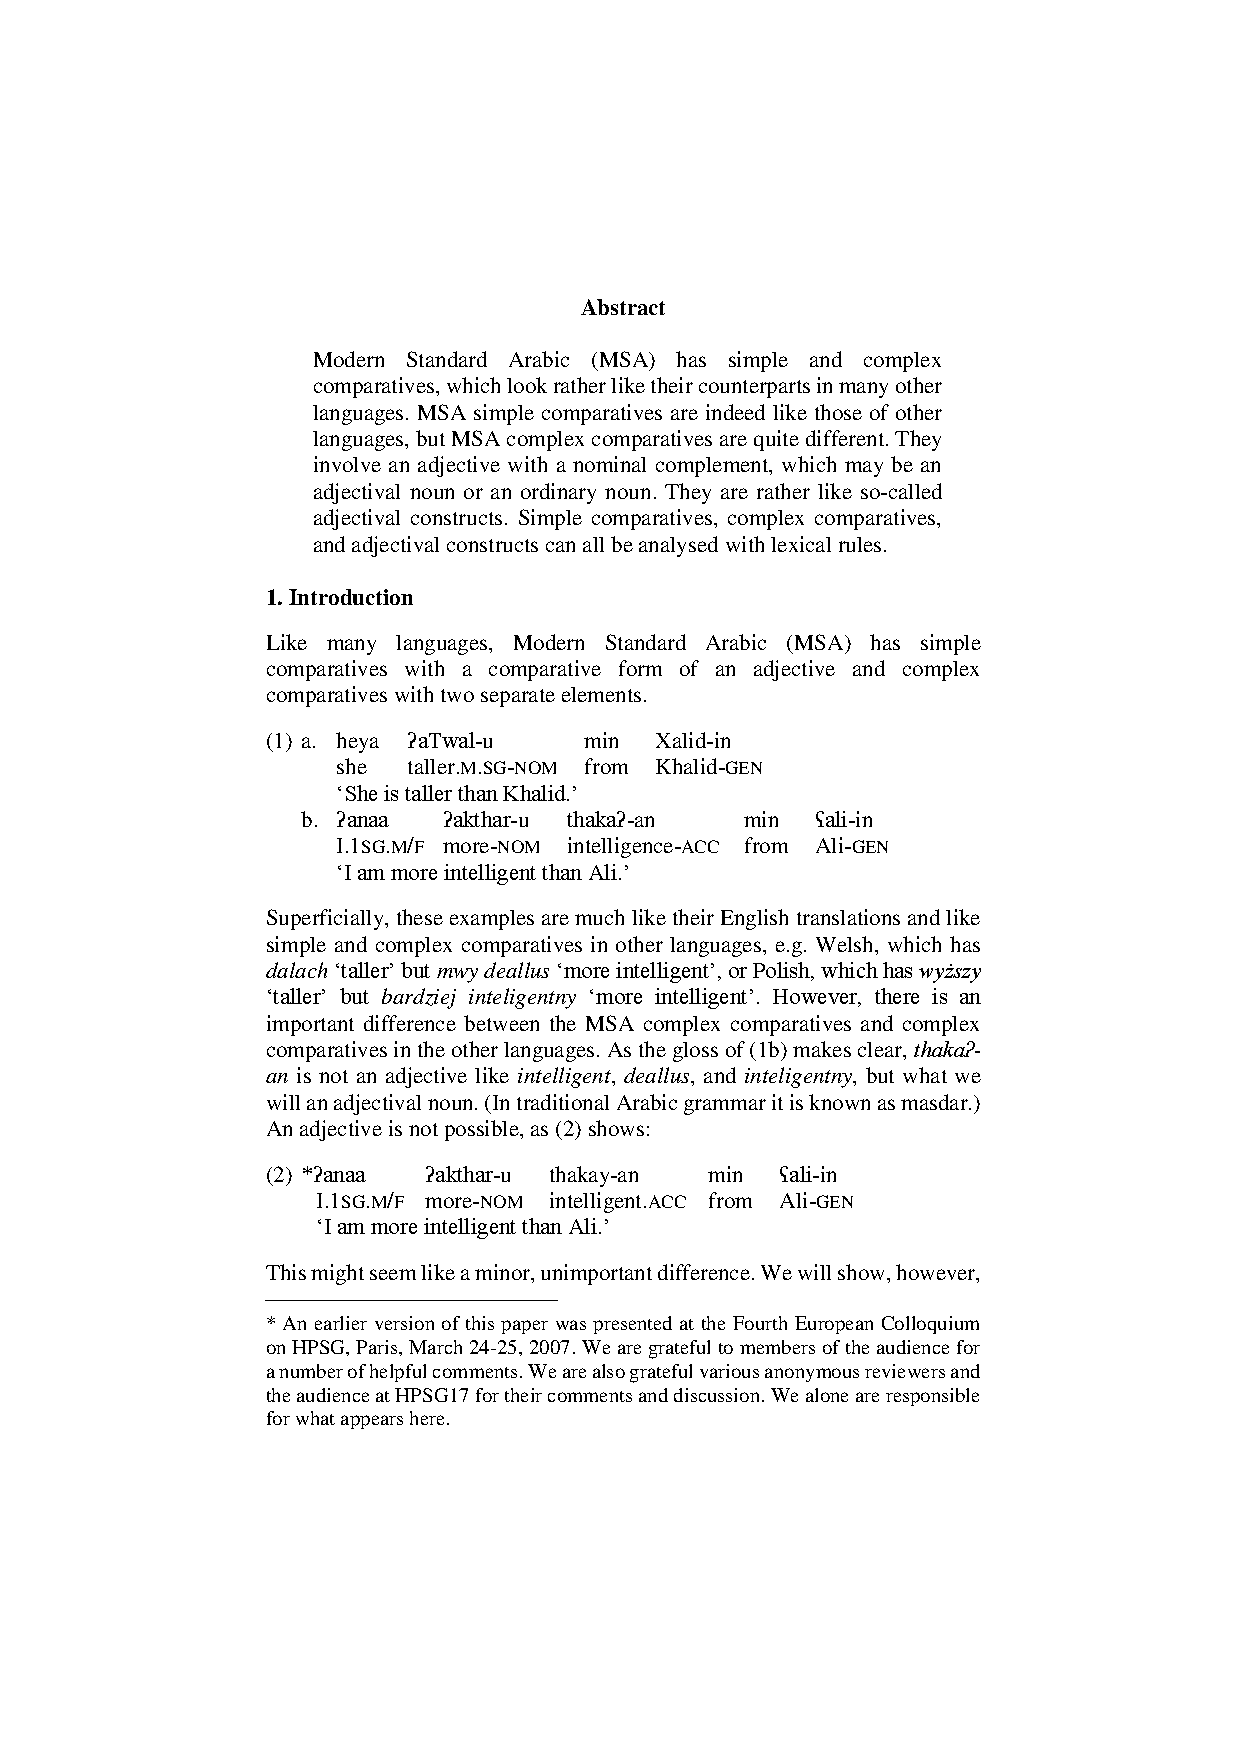
\includepdf[pages=-,pagecommand=\thispagestyle{plain}]{Includes/aab.pdf}
        \setcounter{page}{26}
        \phantomsection
        \addcontentsline{toc}{section}{Aixiu An, Anne Abeill{\'e}: Agreement and interpretation of binominals in French}
\thispagestyle{empty}

\begin{center}
  {\huge\bfseries Agreement and interpretation of binominals in French\par}

  \bigskip

~\\
\begingroup
\setlength{\leftskip}{0pt plus 1fill}
\setlength{\rightskip}{0pt plus 1fill}
\setlength{\parindent}{0pt}
\setlength{\parfillskip}{0pt}
  \formatauthor{Aixiu An}{\begin{tabular}{@{}c@{}}LLF, University Paris Diderot\end{tabular}}
\formatauthor{Anne Abeillé}{\begin{tabular}{@{}c@{}}LLF, University Paris Diderot\end{tabular}}

\par\endgroup

  \vspace*{8ex}

  Proceedings of the 24th International Conference on\par Head-Driven Phrase Structure Grammar

  \bigskip

  University of Kentucky, Lexington

  \medskip

  Stefan Müller (Editor)

  \medskip

  2017

  \medskip

  CSLI Publications

  \medskip

  pages 26--43

  \medskip

  \url{http://csli-publications.stanford.edu/HPSG/2017}
\end{center}
\vfill

\noindent
Keywords: binominals, agreement, HPSG


\vfill
\noindent
% APA Style
An, Aixiu, \& Abeillé, Anne. 2017. Agreement and interpretation of binominals in French. In Müller, Stefan (Ed.), \emph{{Proceedings of the 24th International Conference on Head-Driven Phrase Structure Grammar, University of Kentucky, Lexington}}, 26--43. Stanford,
CA: CSLI Publications. \hfill\href{http://creativecommons.org/licenses/by/4.0/}{\includegraphics[height=.75em]{Includes/ccby.eps}}

\newpage
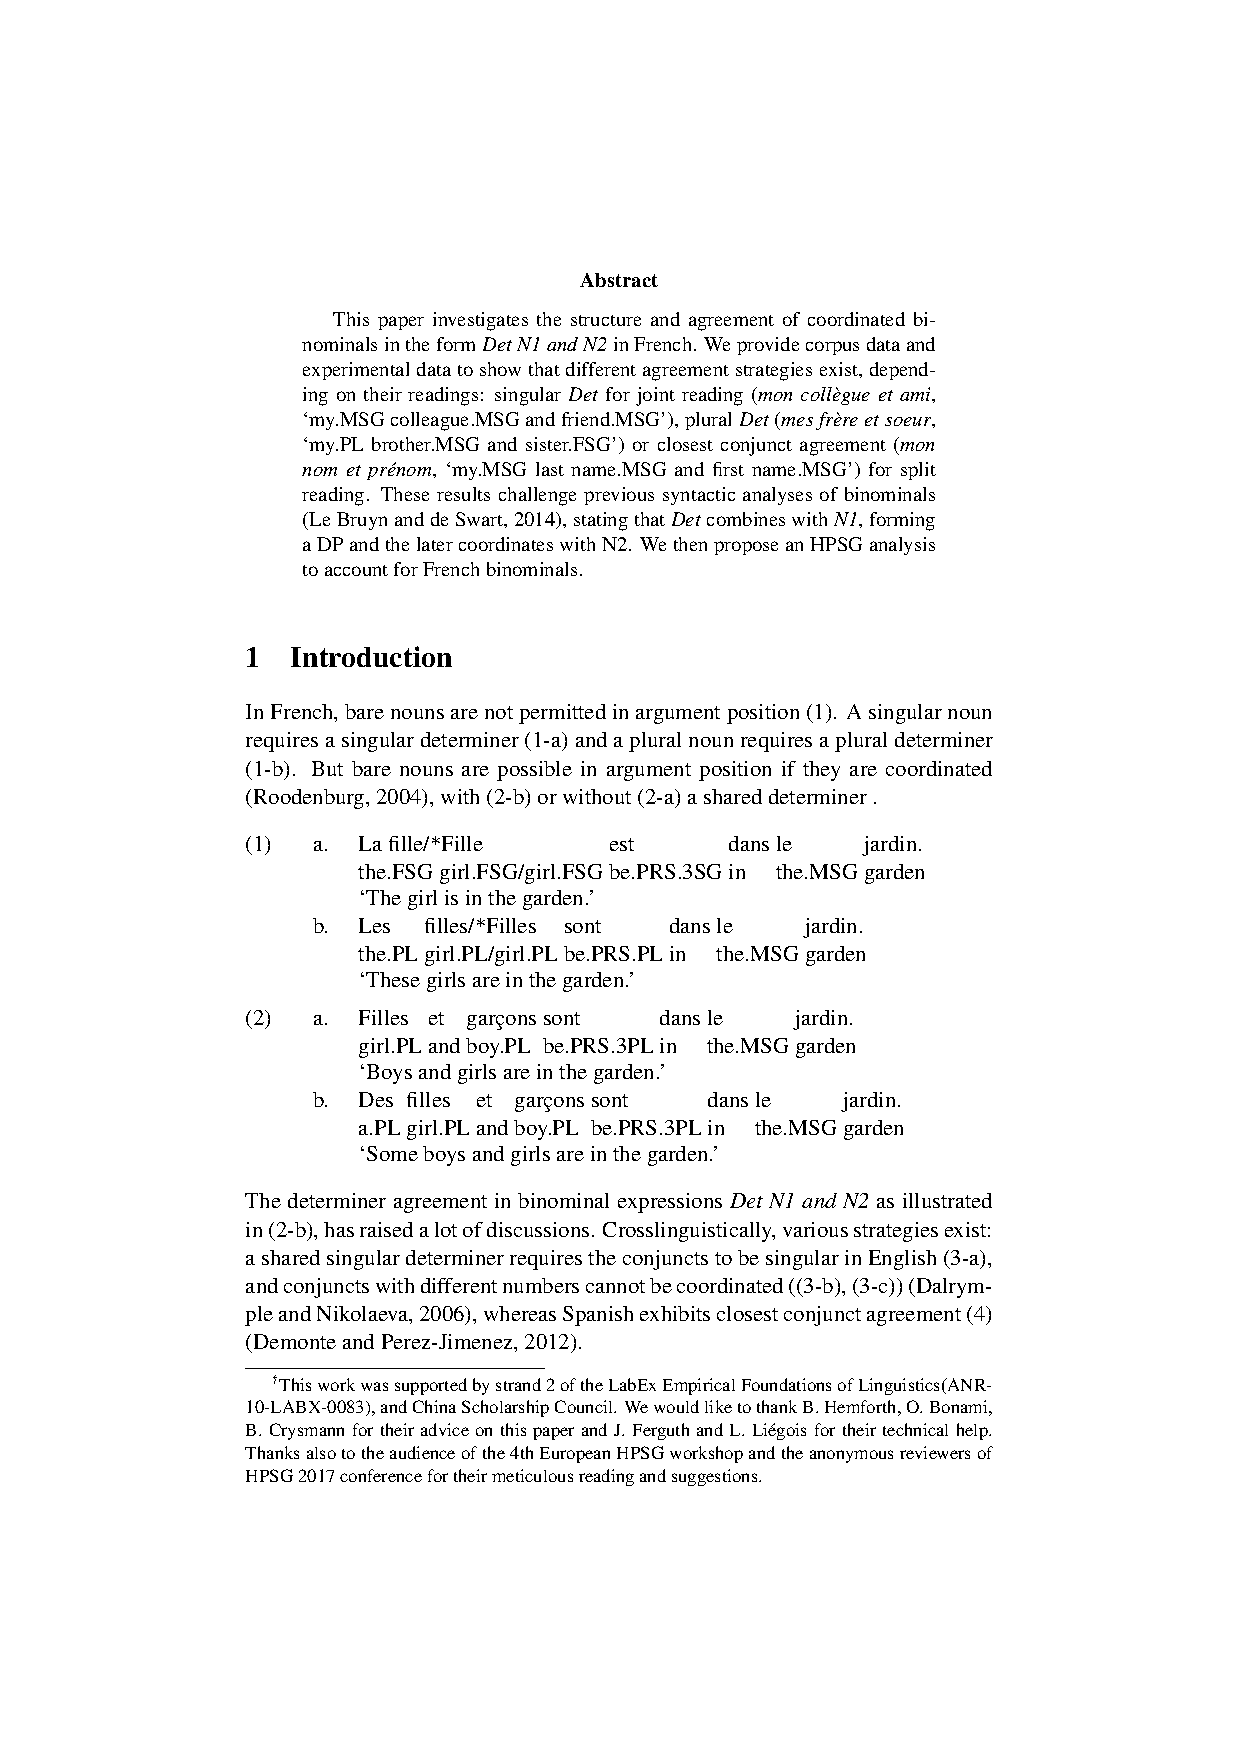
\includepdf[pages=-,pagecommand=\thispagestyle{plain}]{Includes/an-abeille.pdf}
        \setcounter{page}{44}
        \phantomsection
        \addcontentsline{toc}{section}{Tali Arad Greshler, Nurit Melnik: Backward control in Modern Standard Arabic}
\thispagestyle{empty}

\begin{center}
  {\huge\bfseries Backward control in Modern Standard Arabic\par}

  \bigskip

~\\
\begingroup
\setlength{\leftskip}{0pt plus 1fill}
\setlength{\rightskip}{0pt plus 1fill}
\setlength{\parindent}{0pt}
\setlength{\parfillskip}{0pt}
  \formatauthor{Tali Arad Greshler}{\begin{tabular}{@{}c@{}}University of Haifa\end{tabular}}
\formatauthor{Nurit Melnik}{\begin{tabular}{@{}c@{}}The Open University
of Israel\end{tabular}}

\par\endgroup

  \vspace*{8ex}

  Proceedings of the 24th International Conference on\par Head-Driven Phrase Structure Grammar

  \bigskip

  University of Kentucky, Lexington

  \medskip

  Stefan Müller (Editor)

  \medskip

  2017

  \medskip

  CSLI Publications

  \medskip

  pages 44--60

  \medskip

  \url{http://csli-publications.stanford.edu/HPSG/2017}
\end{center}
\vfill

\noindent
Keywords: Modern Standard Arabic, subjunctives, control, complex predicates


\vfill
\noindent
% APA Style
Arad Greshler, Tali, \& Melnik, Nurit. 2017. Backward control in Modern Standard Arabic. In Müller, Stefan (Ed.), \emph{{Proceedings of the 24th International Conference on Head-Driven Phrase Structure Grammar, University of Kentucky, Lexington}}, 44--60. Stanford,
CA: CSLI Publications. \hfill\href{http://creativecommons.org/licenses/by/4.0/}{\includegraphics[height=.75em]{Includes/ccby.eps}}

\newpage
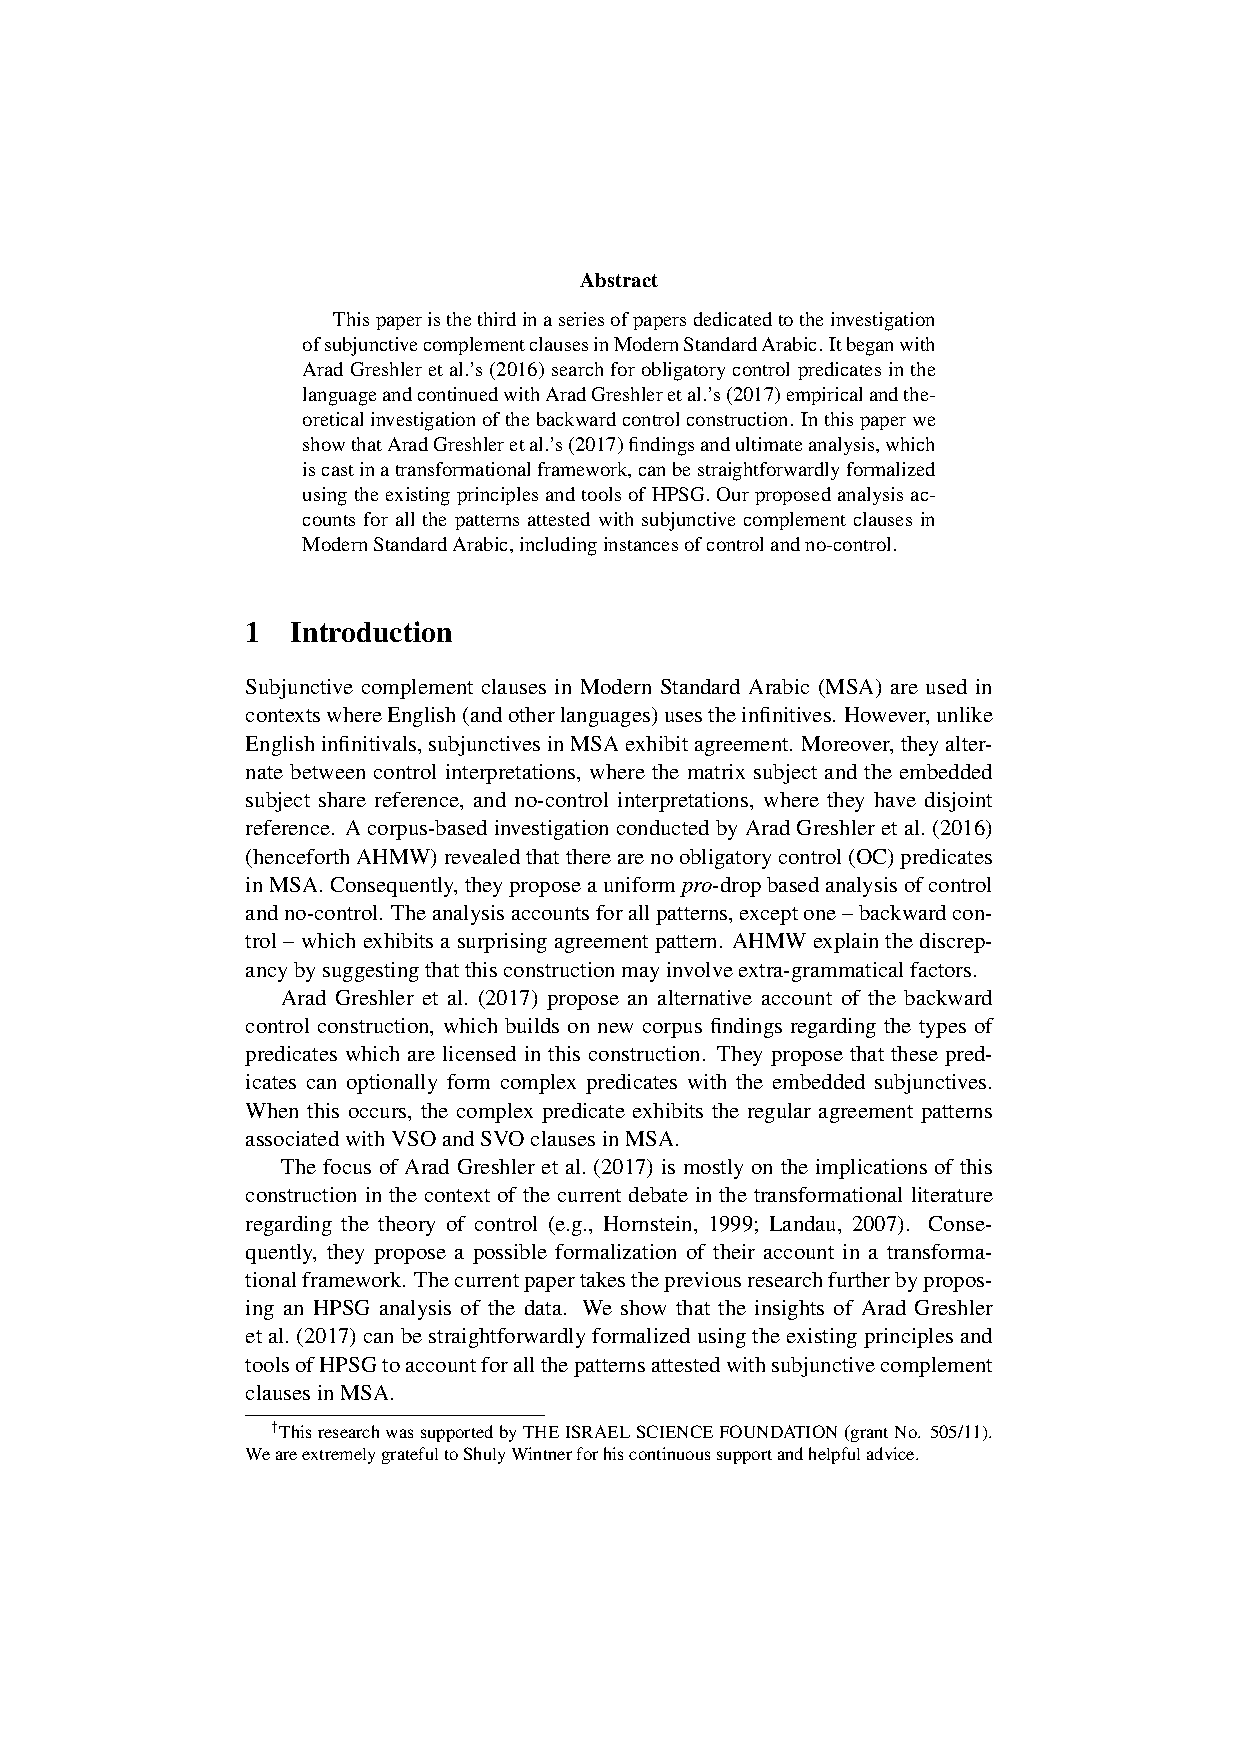
\includepdf[pages=-,pagecommand=\thispagestyle{plain}]{Includes/aradgreshler-melnik.pdf}
        \setcounter{page}{61}
        \phantomsection
        \addcontentsline{toc}{section}{Douglas Ball: ``VP'' Adverbs without a VP:\\ The syntax of adverbs in Tongan}
\thispagestyle{empty}

\begin{center}
  {\huge\bfseries ``VP'' Adverbs without a VP:\par The syntax of adverbs in Tongan\par}

  \bigskip

~\\
\begingroup
\setlength{\leftskip}{0pt plus 1fill}
\setlength{\rightskip}{0pt plus 1fill}
\setlength{\parindent}{0pt}
\setlength{\parfillskip}{0pt}
  \formatauthor{Douglas Ball}{\begin{tabular}{@{}c@{}}Truman State University\end{tabular}}

\par\endgroup

  \vspace*{8ex}

  Proceedings of the 24th International Conference on\par Head-Driven Phrase Structure Grammar

  \bigskip

  University of Kentucky, Lexington

  \medskip

  Stefan Müller (Editor)

  \medskip

  2017

  \medskip

  CSLI Publications

  \medskip

  pages 61--81

  \medskip

  \url{http://csli-publications.stanford.edu/HPSG/2017}
\end{center}
\vfill

\noindent
Keywords: Tongan, Polynesian, Adverbs, Adjunct Syntax, HPSG


\vfill
\noindent
% APA Style
Ball, Douglas. 2017. ``VP'' Adverbs without a VP:  The syntax of adverbs in Tongan. In Müller, Stefan (Ed.), \emph{{Proceedings of the 24th International Conference on Head-Driven Phrase Structure Grammar, University of Kentucky, Lexington}}, 61--81. Stanford,
CA: CSLI Publications. \hfill\href{http://creativecommons.org/licenses/by/4.0/}{\includegraphics[height=.75em]{Includes/ccby.eps}}

\newpage
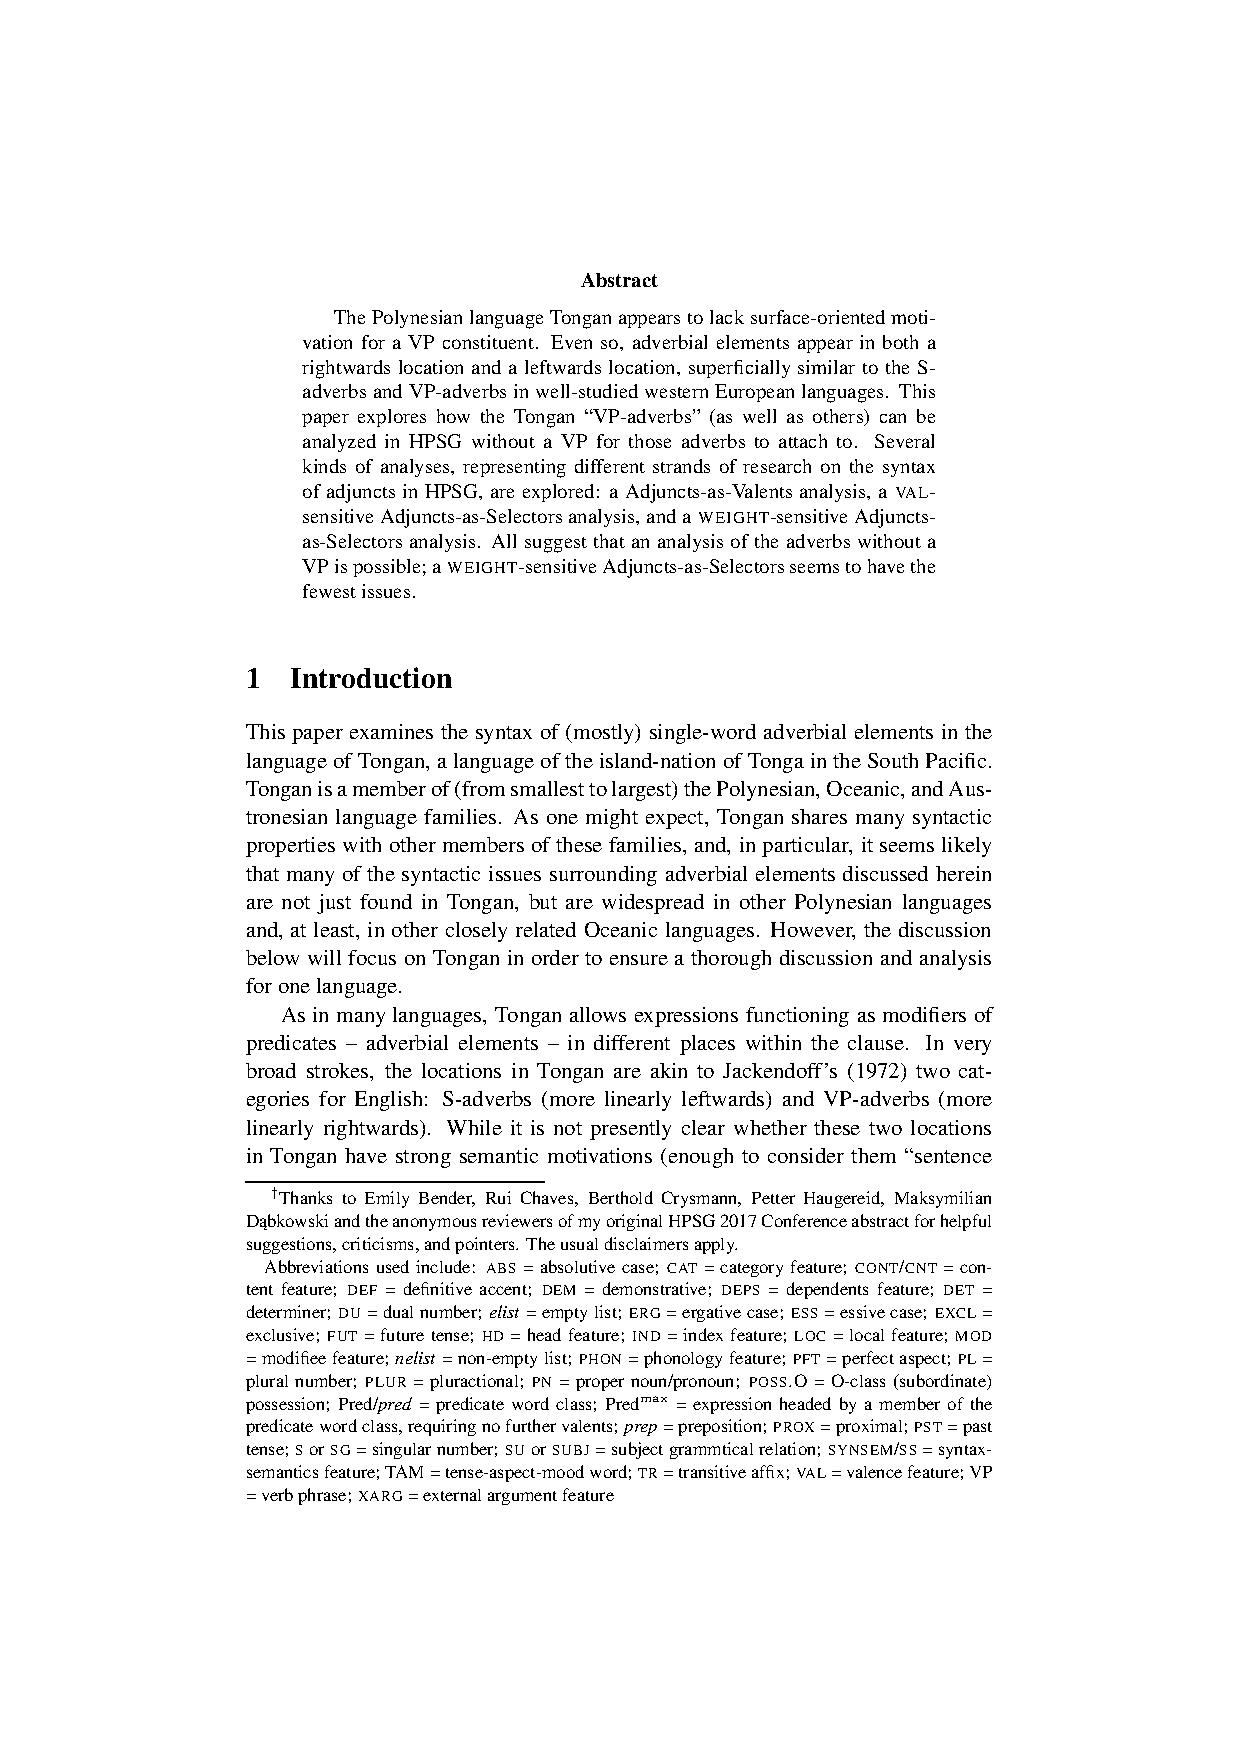
\includepdf[pages=-,pagecommand=\thispagestyle{plain}]{Includes/ball.pdf}
        \setcounter{page}{82}
        \phantomsection
        \addcontentsline{toc}{section}{Robert D. Borsley: Explanations and `Engineering Solutions'? Aspects of the Relation between Minimalism and HPSG}
\thispagestyle{empty}

\begin{center}
  {\huge\bfseries Explanations and `Engineering Solutions'? Aspects of the Relation between Minimalism and HPSG\par}

  \bigskip

~\\
\begingroup
\setlength{\leftskip}{0pt plus 1fill}
\setlength{\rightskip}{0pt plus 1fill}
\setlength{\parindent}{0pt}
\setlength{\parfillskip}{0pt}
  \formatauthor{Robert D. Borsley}{\begin{tabular}{@{}c@{}}University of Essex\end{tabular}}

\par\endgroup

  \vspace*{8ex}

  Proceedings of the 24th International Conference on\par Head-Driven Phrase Structure Grammar

  \bigskip

  University of Kentucky, Lexington

  \medskip

  Stefan Müller (Editor)

  \medskip

  2017

  \medskip

  CSLI Publications

  \medskip

  pages 82--102

  \medskip

  \url{http://csli-publications.stanford.edu/HPSG/2017}
\end{center}
\vfill

\noindent
Keywords: Minimalism, the lexicon and syntax, Internal Merge, SLASH


\vfill
\noindent
% APA Style
Borsley, Robert D. 2017. Explanations and `Engineering Solutions'? Aspects of the Relation between Minimalism and HPSG. In Müller, Stefan (Ed.), \emph{{Proceedings of the 24th International Conference on Head-Driven Phrase Structure Grammar, University of Kentucky, Lexington}}, 82--102. Stanford,
CA: CSLI Publications. \hfill\href{http://creativecommons.org/licenses/by/4.0/}{\includegraphics[height=.75em]{Includes/ccby.eps}}

\newpage
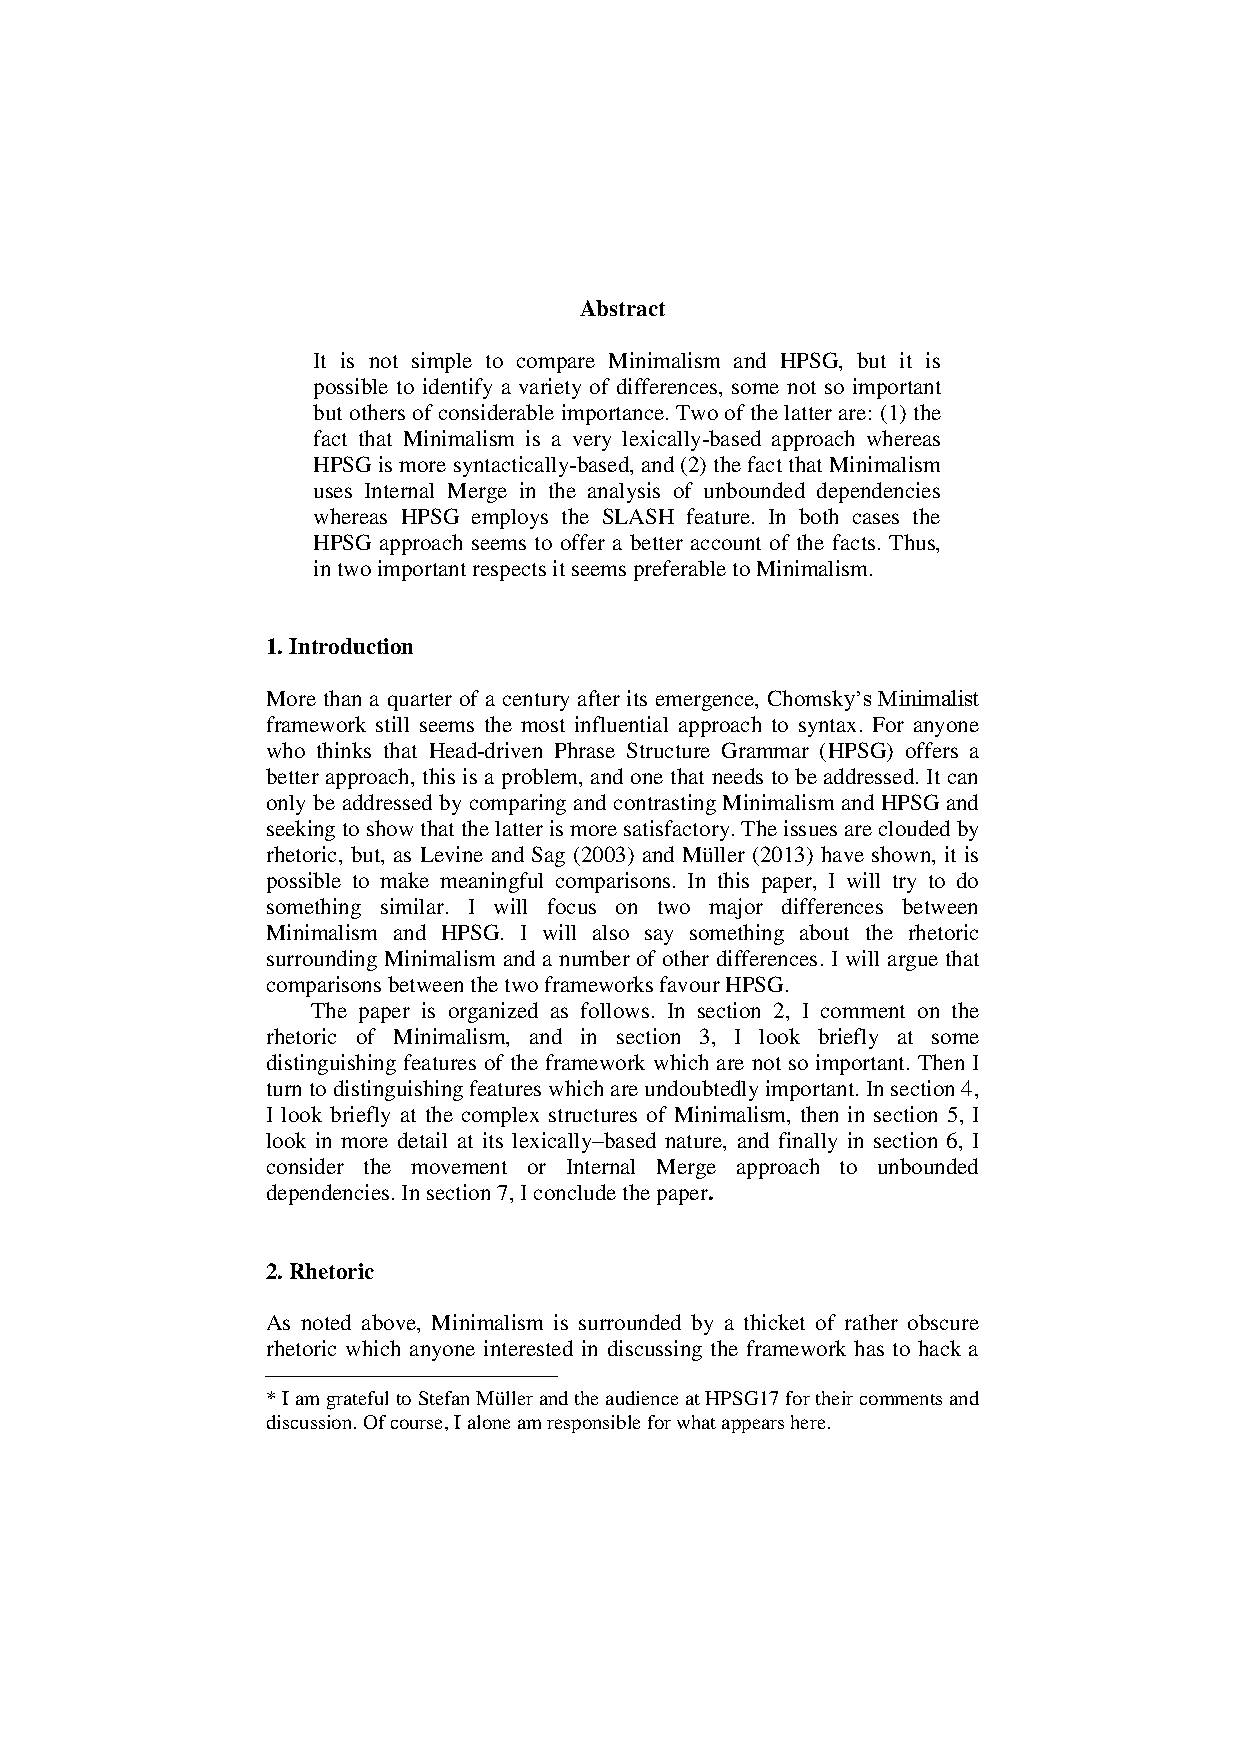
\includepdf[pages=-,pagecommand=\thispagestyle{plain}]{Includes/borsley.pdf}
        \setcounter{page}{103}
        \phantomsection
        \addcontentsline{toc}{section}{George Aaron Broadwell: Parallel affix blocks in Choctaw}
\thispagestyle{empty}

\begin{center}
  {\huge\bfseries Parallel affix blocks in Choctaw\par}

  \bigskip

~\\
\begingroup
\setlength{\leftskip}{0pt plus 1fill}
\setlength{\rightskip}{0pt plus 1fill}
\setlength{\parindent}{0pt}
\setlength{\parfillskip}{0pt}
  \formatauthor{George Aaron Broadwell}{\begin{tabular}{@{}c@{}}University of Florida\end{tabular}}

\par\endgroup

  \vspace*{8ex}

  Proceedings of the 24th International Conference on\par Head-Driven Phrase Structure Grammar

  \bigskip

  University of Kentucky, Lexington

  \medskip

  Stefan Müller (Editor)

  \medskip

  2017

  \medskip

  CSLI Publications

  \medskip

  pages 103--119

  \medskip

  \url{http://csli-publications.stanford.edu/HPSG/2017}
\end{center}
\vfill

\noindent
Keywords: agreement, exponence, morphotactics, information-based morphology, paradigm function morphology


\vfill
\noindent
% APA Style
Broadwell, George Aaron. 2017. Parallel affix blocks in Choctaw. In Müller, Stefan (Ed.), \emph{{Proceedings of the 24th International Conference on Head-Driven Phrase Structure Grammar, University of Kentucky, Lexington}}, 103--119. Stanford,
CA: CSLI Publications. \hfill\href{http://creativecommons.org/licenses/by/4.0/}{\includegraphics[height=.75em]{Includes/ccby.eps}}

\newpage
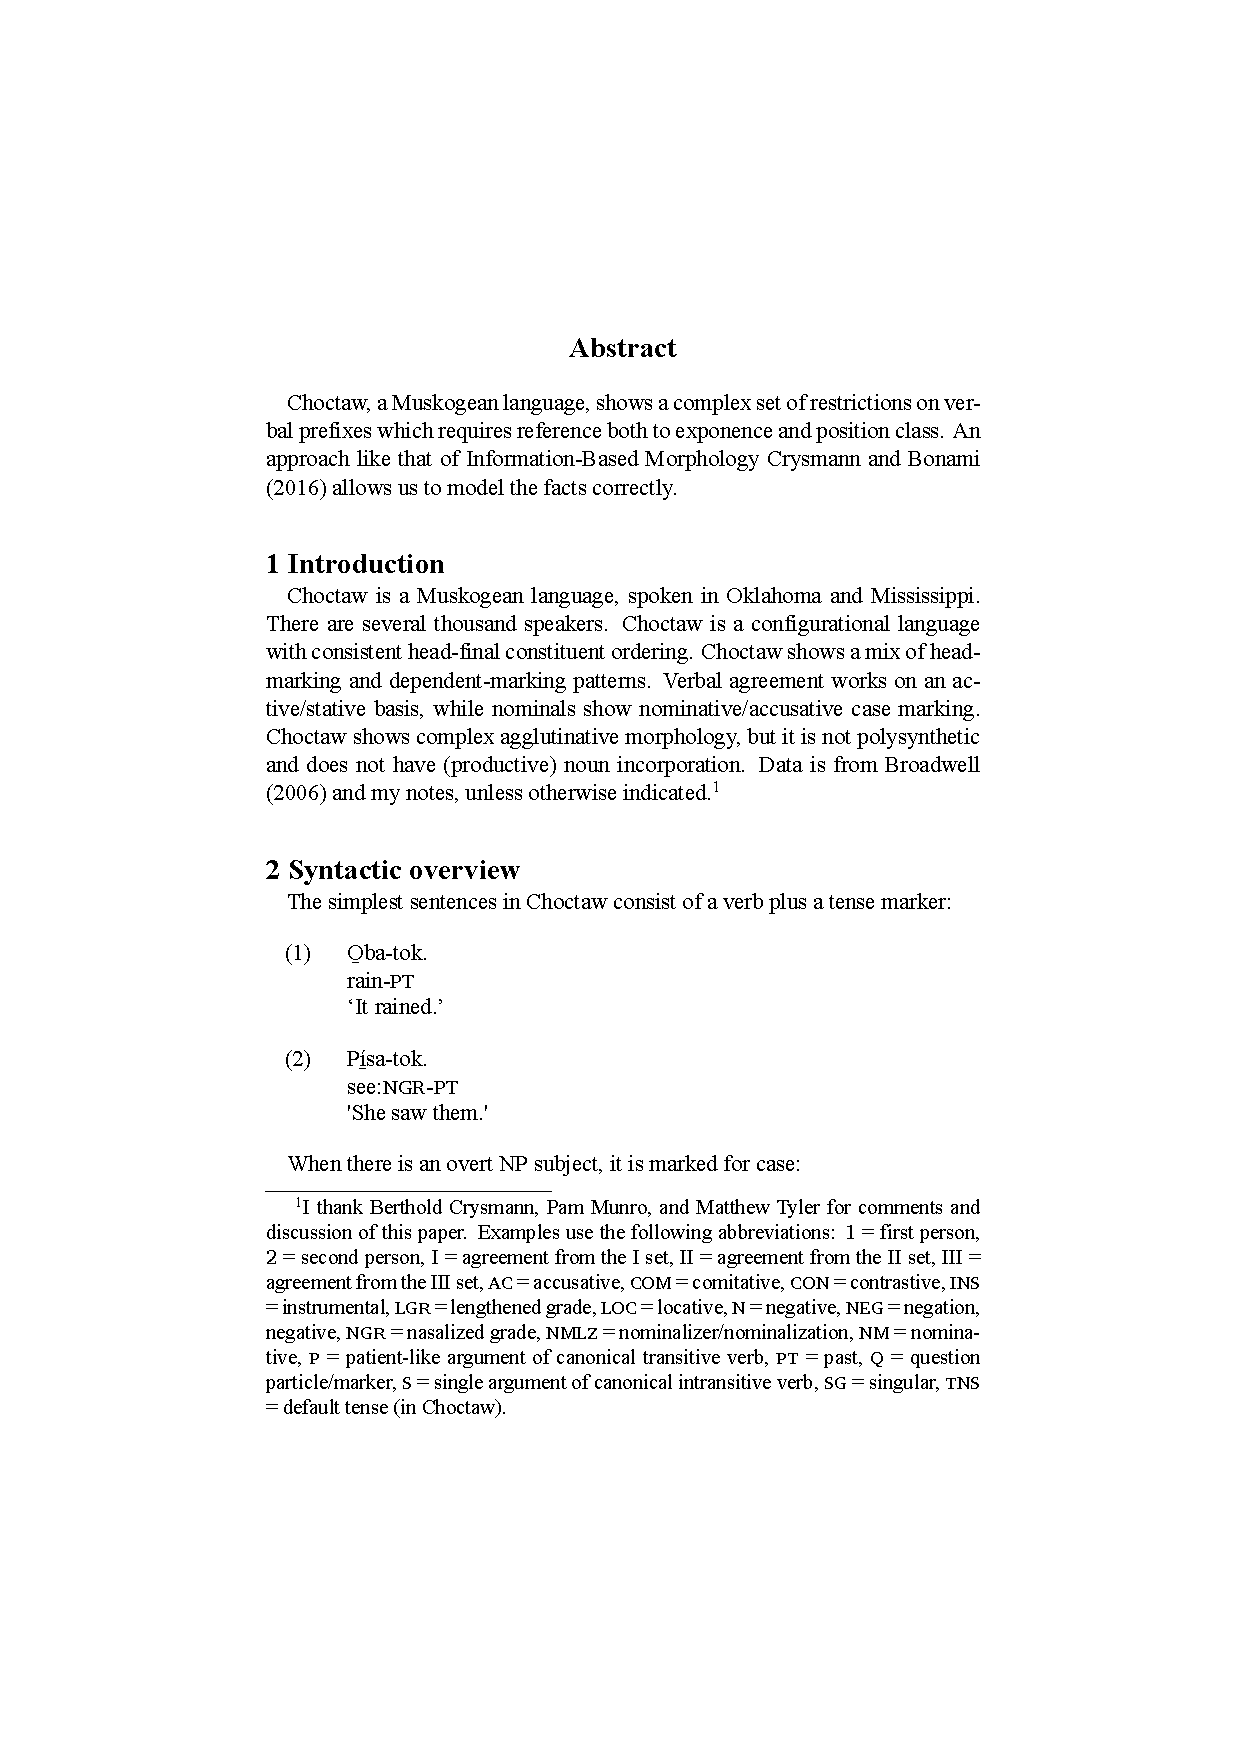
\includepdf[pages=-,pagecommand=\thispagestyle{plain}]{Includes/broadwell.pdf}
        \setcounter{page}{120}
        \phantomsection
        \addcontentsline{toc}{section}{Berthold Crysmann: Resumption and case: A new take on Modern Standard Arabic}
\thispagestyle{empty}

\begin{center}
  {\huge\bfseries Resumption and case: A new take on Modern Standard Arabic\par}

  \bigskip

~\\
\begingroup
\setlength{\leftskip}{0pt plus 1fill}
\setlength{\rightskip}{0pt plus 1fill}
\setlength{\parindent}{0pt}
\setlength{\parfillskip}{0pt}
  \formatauthor{Berthold Crysmann}{\begin{tabular}{@{}c@{}}Laboratoire de linguistique formelle, CNRS\end{tabular}}

\par\endgroup

  \vspace*{8ex}

  Proceedings of the 24th International Conference on\par Head-Driven Phrase Structure Grammar

  \bigskip

  University of Kentucky, Lexington

  \medskip

  Stefan Müller (Editor)

  \medskip

  2017

  \medskip

  CSLI Publications

  \medskip

  pages 120--140

  \medskip

  \url{http://csli-publications.stanford.edu/HPSG/2017}
\end{center}
\vfill

\noindent
Keywords: Resumption, Extraction, Modern Standard Arabic, Across-the-board, Case, Gap


\vfill
\noindent
% APA Style
Crysmann, Berthold. 2017. Resumption and case: A new take on Modern Standard Arabic. In Müller, Stefan (Ed.), \emph{{Proceedings of the 24th International Conference on Head-Driven Phrase Structure Grammar, University of Kentucky, Lexington}}, 120--140. Stanford,
CA: CSLI Publications. \hfill\href{http://creativecommons.org/licenses/by/4.0/}{\includegraphics[height=.75em]{Includes/ccby.eps}}

\newpage
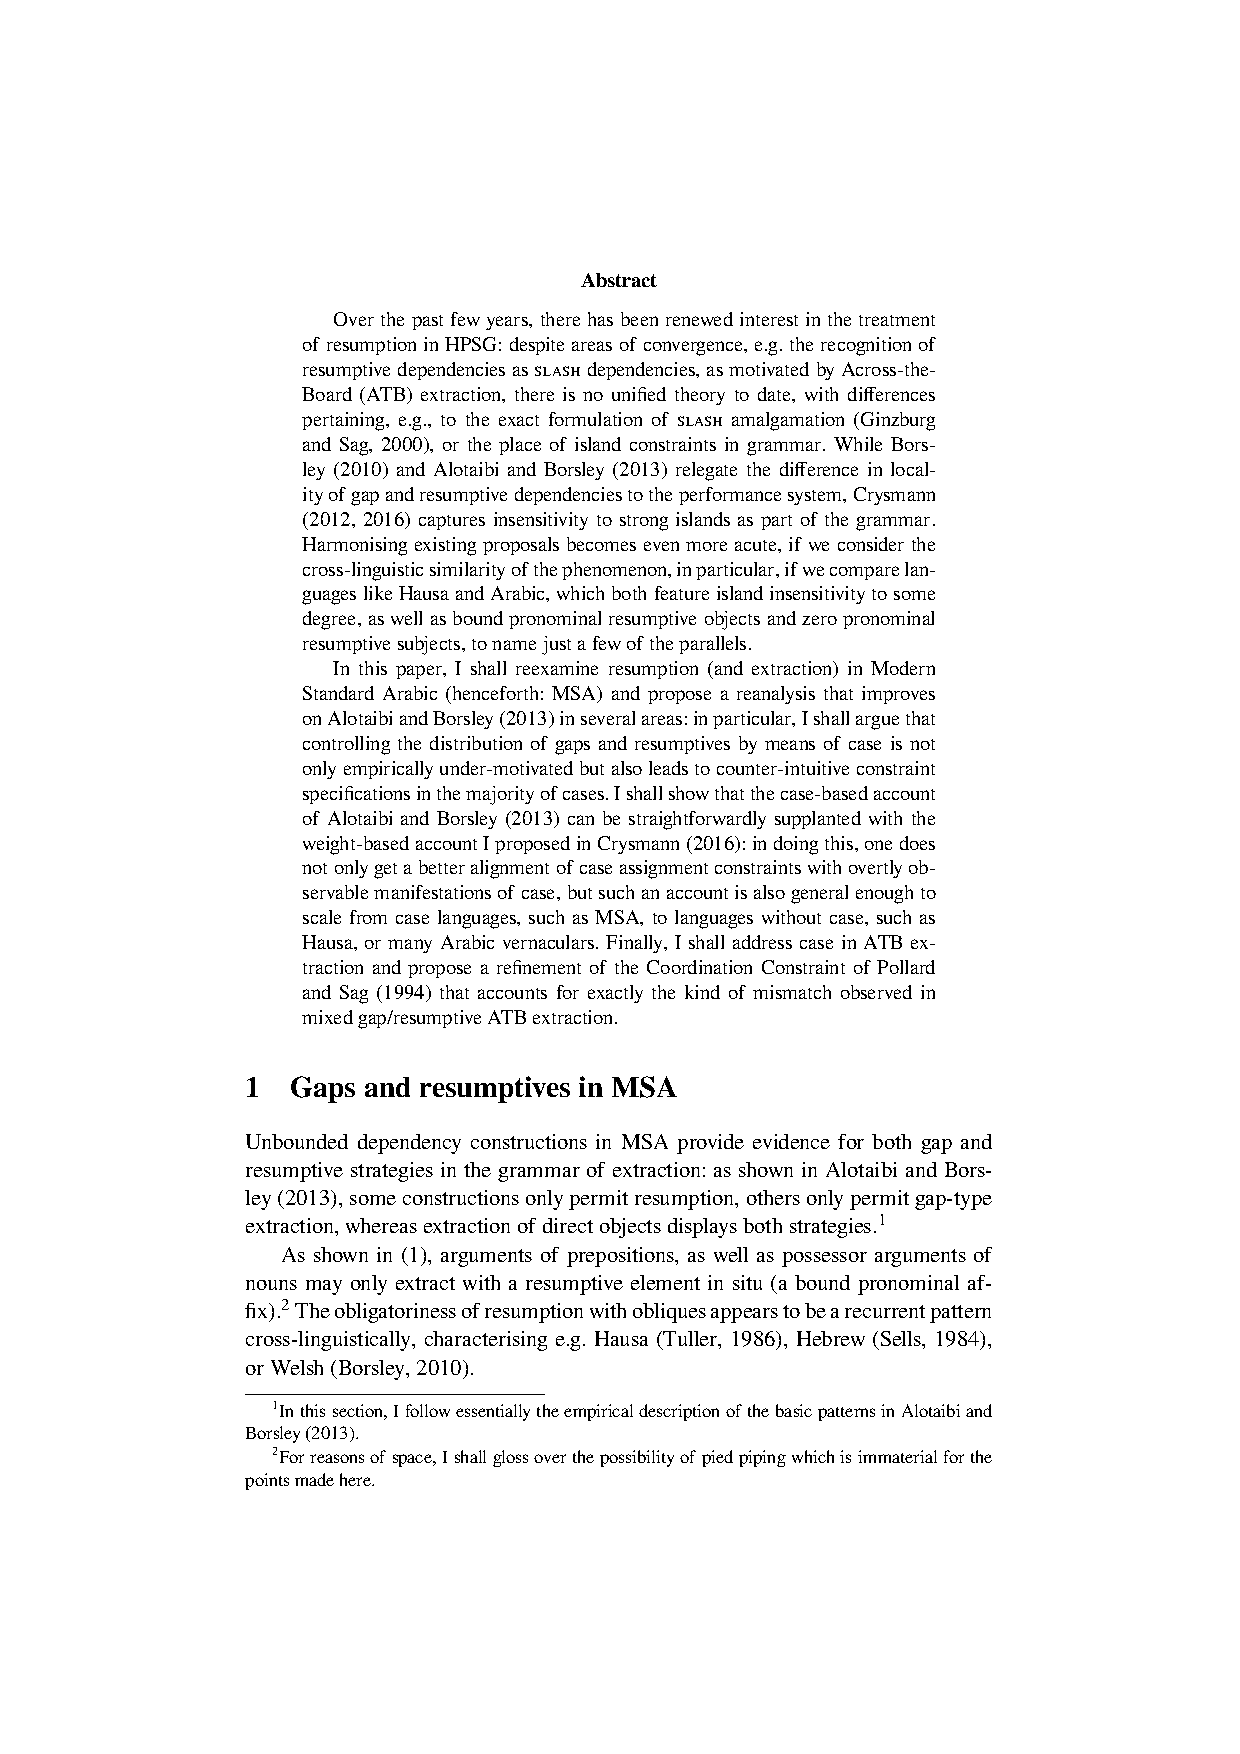
\includepdf[pages=-,pagecommand=\thispagestyle{plain}]{Includes/crysmann.pdf}
        \setcounter{page}{141}
        \phantomsection
        \addcontentsline{toc}{section}{Berthold Crysmann, Olivier Bonami: Atomistic and holistic exponence in Information-based Morphology}
\thispagestyle{empty}

\begin{center}
  {\huge\bfseries Atomistic and holistic exponence in Information-based Morphology\par}

  \bigskip

~\\
\begingroup
\setlength{\leftskip}{0pt plus 1fill}
\setlength{\rightskip}{0pt plus 1fill}
\setlength{\parindent}{0pt}
\setlength{\parfillskip}{0pt}
  \formatauthor{Berthold Crysmann}{\begin{tabular}{@{}c@{}}Laboratoire de linguistique formelle, CNRS\end{tabular}}
\formatauthor{Olivier Bonami}{\begin{tabular}{@{}c@{}}Laboratoire de linguistique formelle, U Paris-Diderot\end{tabular}}

\par\endgroup

  \vspace*{8ex}

  Proceedings of the 24th International Conference on\par Head-Driven Phrase Structure Grammar

  \bigskip

  University of Kentucky, Lexington

  \medskip

  Stefan Müller (Editor)

  \medskip

  2017

  \medskip

  CSLI Publications

  \medskip

  pages 141--161

  \medskip

  \url{http://csli-publications.stanford.edu/HPSG/2017}
\end{center}
\vfill

\noindent
Keywords: Inflection, Exponence, Realisational Morphology, Estonian, Swahili


\vfill
\noindent
% APA Style
Crysmann, Berthold, \& Bonami, Olivier. 2017. Atomistic and holistic exponence in Information-based Morphology. In Müller, Stefan (Ed.), \emph{{Proceedings of the 24th International Conference on Head-Driven Phrase Structure Grammar, University of Kentucky, Lexington}}, 141--161. Stanford,
CA: CSLI Publications. \hfill\href{http://creativecommons.org/licenses/by/4.0/}{\includegraphics[height=.75em]{Includes/ccby.eps}}

\newpage
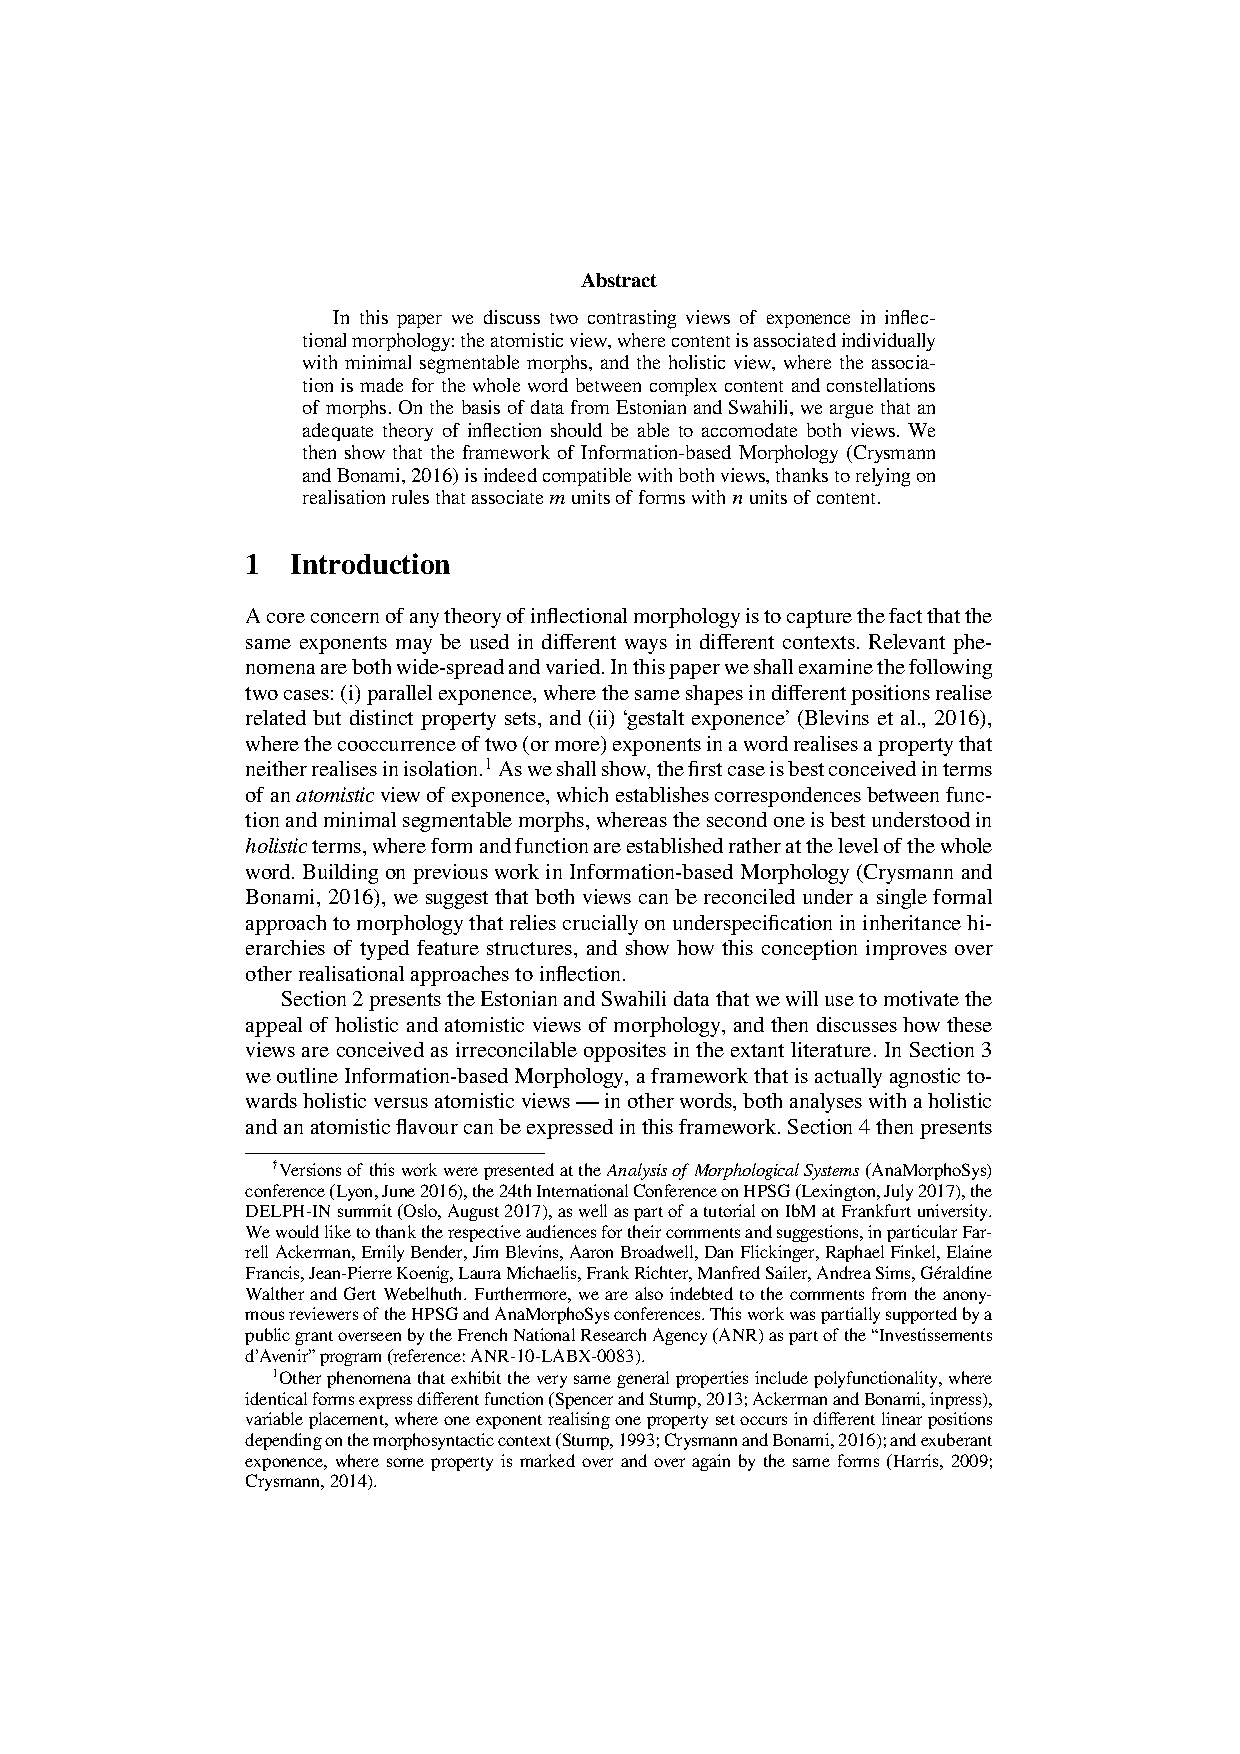
\includepdf[pages=-,pagecommand=\thispagestyle{plain}]{Includes/crysmann-bonami.pdf}
        \setcounter{page}{162}
        \phantomsection
        \addcontentsline{toc}{section}{Maksymilian D\k{a}bkowski: Yucatecan Control and Lexical Categories in SBCG}
\thispagestyle{empty}

\begin{center}
  {\huge\bfseries Yucatecan Control and Lexical Categories in SBCG\par}

  \bigskip

~\\
\begingroup
\setlength{\leftskip}{0pt plus 1fill}
\setlength{\rightskip}{0pt plus 1fill}
\setlength{\parindent}{0pt}
\setlength{\parfillskip}{0pt}
  \formatauthor{Maksymilian Dąbkowski}{\begin{tabular}{@{}c@{}}Brown University\end{tabular}}

\par\endgroup

  \vspace*{8ex}

  Proceedings of the 24th International Conference on\par Head-Driven Phrase Structure Grammar

  \bigskip

  University of Kentucky, Lexington

  \medskip

  Stefan Müller (Editor)

  \medskip

  2017

  \medskip

  CSLI Publications

  \medskip

  pages 162--178

  \medskip

  \url{http://csli-publications.stanford.edu/HPSG/2017}
\end{center}
\vfill

\noindent
Keywords: Yucatec Maya, SBCG, control, lexical categories


\vfill
\noindent
% APA Style
Dąbkowski, Maksymilian. 2017. Yucatecan Control and Lexical Categories in SBCG. In Müller, Stefan (Ed.), \emph{{Proceedings of the 24th International Conference on Head-Driven Phrase Structure Grammar, University of Kentucky, Lexington}}, 162--178. Stanford,
CA: CSLI Publications. \hfill\href{http://creativecommons.org/licenses/by/4.0/}{\includegraphics[height=.75em]{Includes/ccby.eps}}

\newpage
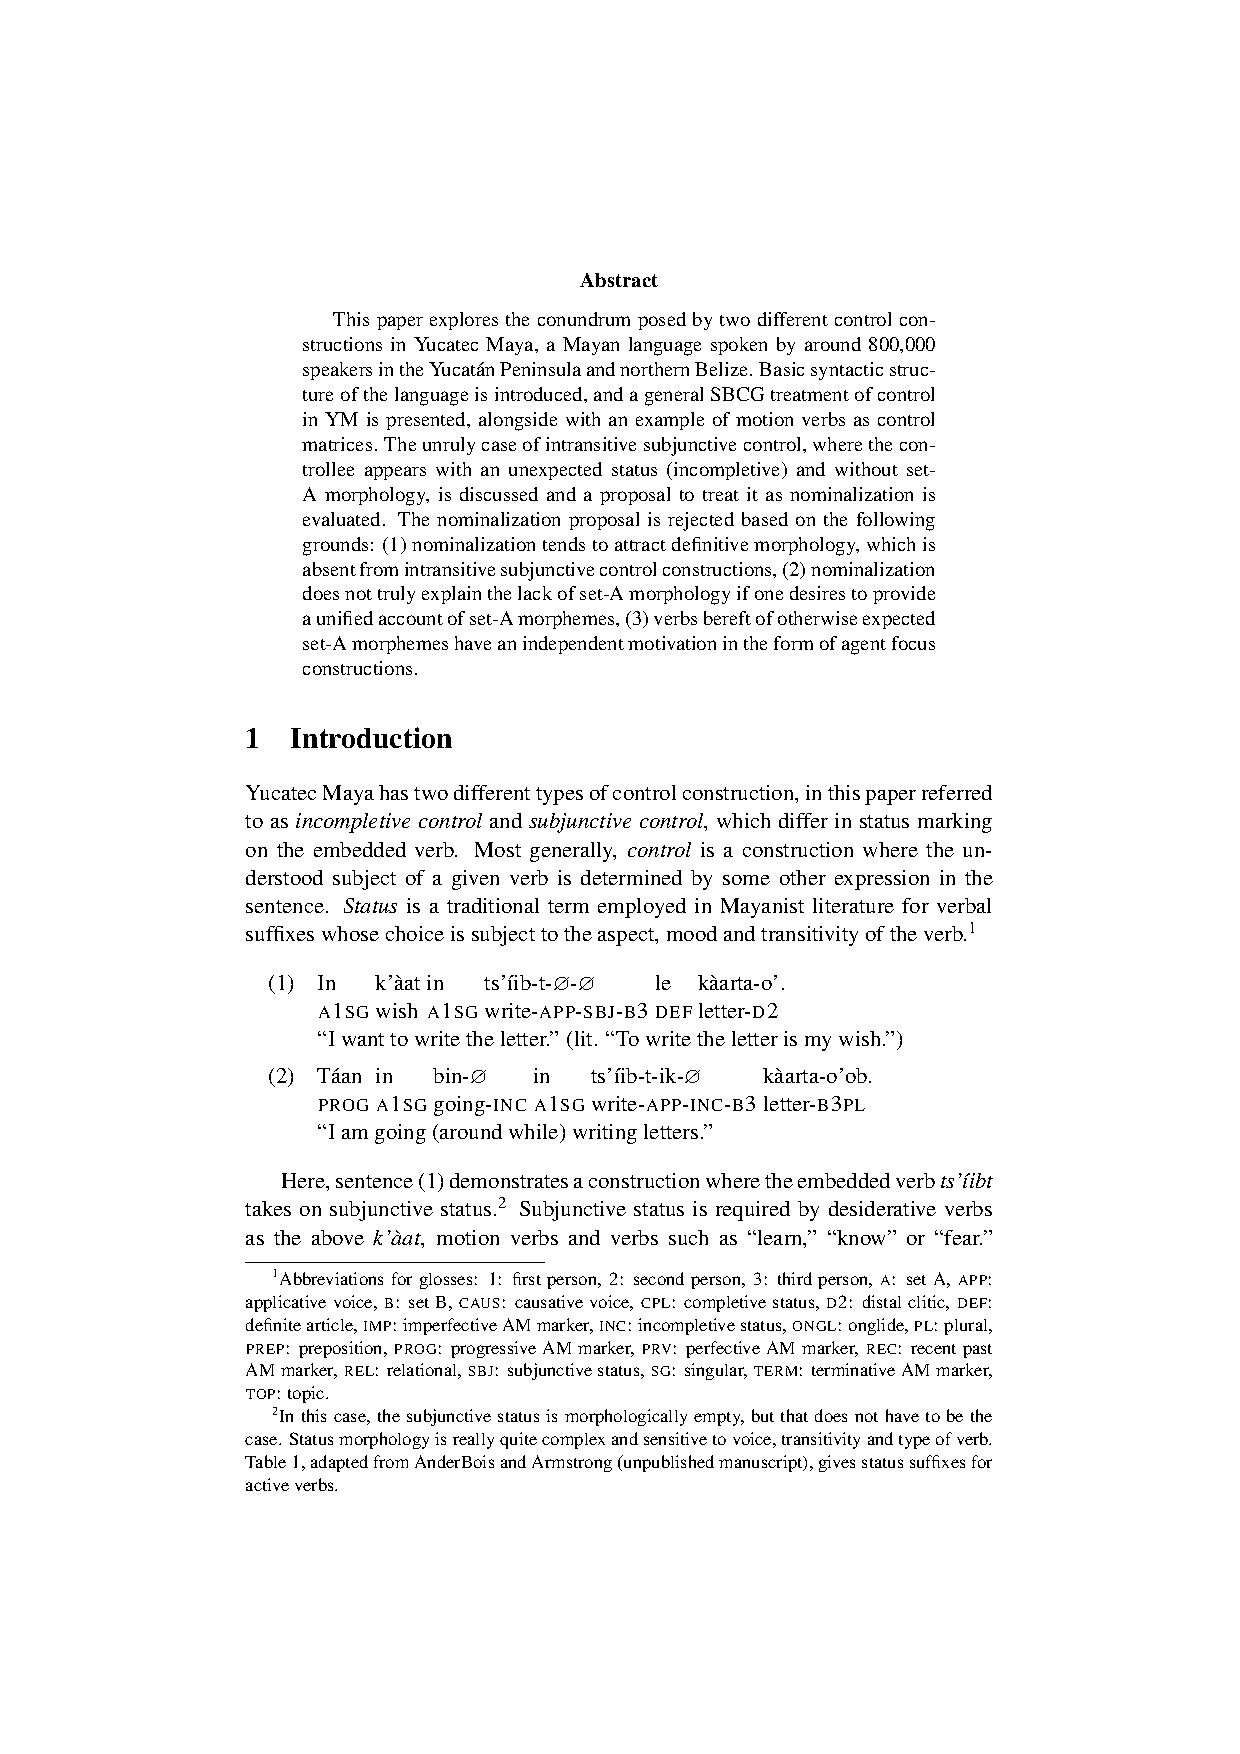
\includepdf[pages=-,pagecommand=\thispagestyle{plain}]{Includes/dabkowski.pdf}
        \setcounter{page}{179}
        \phantomsection
        \addcontentsline{toc}{section}{Petter Haugereid: An incremental approach to gapping and conjunction reduction}
\thispagestyle{empty}

\begin{center}
  {\huge\bfseries An incremental approach to gapping and conjunction reduction\par}

  \bigskip

~\\
\begingroup
\setlength{\leftskip}{0pt plus 1fill}
\setlength{\rightskip}{0pt plus 1fill}
\setlength{\parindent}{0pt}
\setlength{\parfillskip}{0pt}
  \formatauthor{Petter Haugereid}{\begin{tabular}{@{}c@{}}Western Norway University of Applied Sciences\end{tabular}}

\par\endgroup

  \vspace*{8ex}

  Proceedings of the 24th International Conference on\par Head-Driven Phrase Structure Grammar

  \bigskip

  University of Kentucky, Lexington

  \medskip

  Stefan Müller (Editor)

  \medskip

  2017

  \medskip

  CSLI Publications

  \medskip

  pages 179--198

  \medskip

  \url{http://csli-publications.stanford.edu/HPSG/2017}
\end{center}
\vfill

\noindent
Keywords: HPSG, Gapping, Conjunction Reduction, Incremental Parsing


\vfill
\noindent
% APA Style
Haugereid, Petter. 2017. An incremental approach to gapping and conjunction reduction. In Müller, Stefan (Ed.), \emph{{Proceedings of the 24th International Conference on Head-Driven Phrase Structure Grammar, University of Kentucky, Lexington}}, 179--198. Stanford,
CA: CSLI Publications. \hfill\href{http://creativecommons.org/licenses/by/4.0/}{\includegraphics[height=.75em]{Includes/ccby.eps}}

\newpage
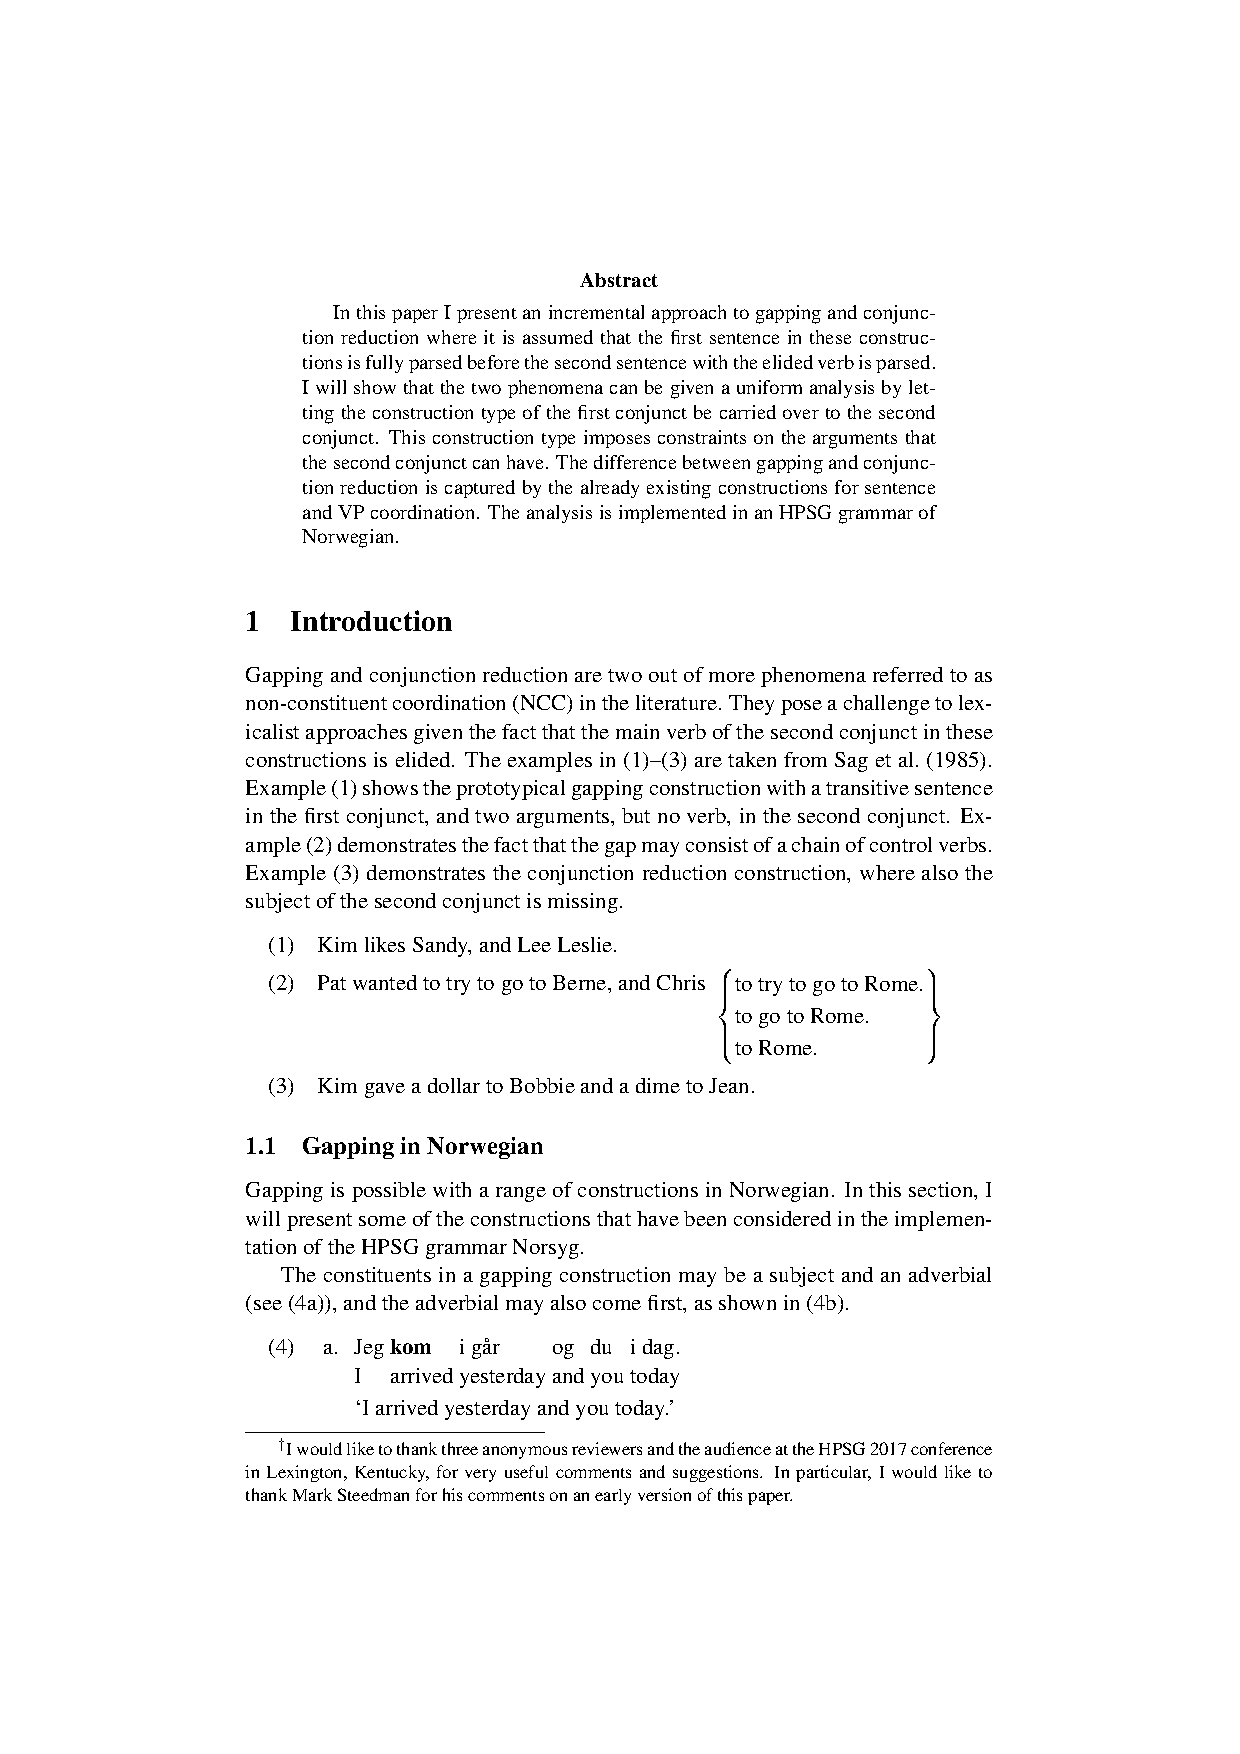
\includepdf[pages=-,pagecommand=\thispagestyle{plain}]{Includes/haugereid.pdf}
        \setcounter{page}{199}
        \phantomsection
        \addcontentsline{toc}{section}{Robert Hepburn-Gray: Against Split Morphology}
\thispagestyle{empty}

\begin{center}
  {\huge\bfseries Against Split Morphology\par}

  \bigskip

~\\
\begingroup
\setlength{\leftskip}{0pt plus 1fill}
\setlength{\rightskip}{0pt plus 1fill}
\setlength{\parindent}{0pt}
\setlength{\parfillskip}{0pt}
  \formatauthor{Robert Hepburn-Gray}{\begin{tabular}{@{}c@{}}University at Buffalo (SUNY)\end{tabular}}

\par\endgroup

  \vspace*{8ex}

  Proceedings of the 24th International Conference on\par Head-Driven Phrase Structure Grammar

  \bigskip

  University of Kentucky, Lexington

  \medskip

  Stefan Müller (Editor)

  \medskip

  2017

  \medskip

  CSLI Publications

  \medskip

  pages 199--211

  \medskip

  \url{http://csli-publications.stanford.edu/HPSG/2017}
\end{center}
\vfill

\noindent
Keywords: SBCG, Word and Paradigm morphology, noun classes, Niger-Congo


\vfill
\noindent
% APA Style
Hepburn-Gray, Robert. 2017. Against Split Morphology. In Müller, Stefan (Ed.), \emph{{Proceedings of the 24th International Conference on Head-Driven Phrase Structure Grammar, University of Kentucky, Lexington}}, 199--211. Stanford,
CA: CSLI Publications. \hfill\href{http://creativecommons.org/licenses/by/4.0/}{\includegraphics[height=.75em]{Includes/ccby.eps}}

\newpage
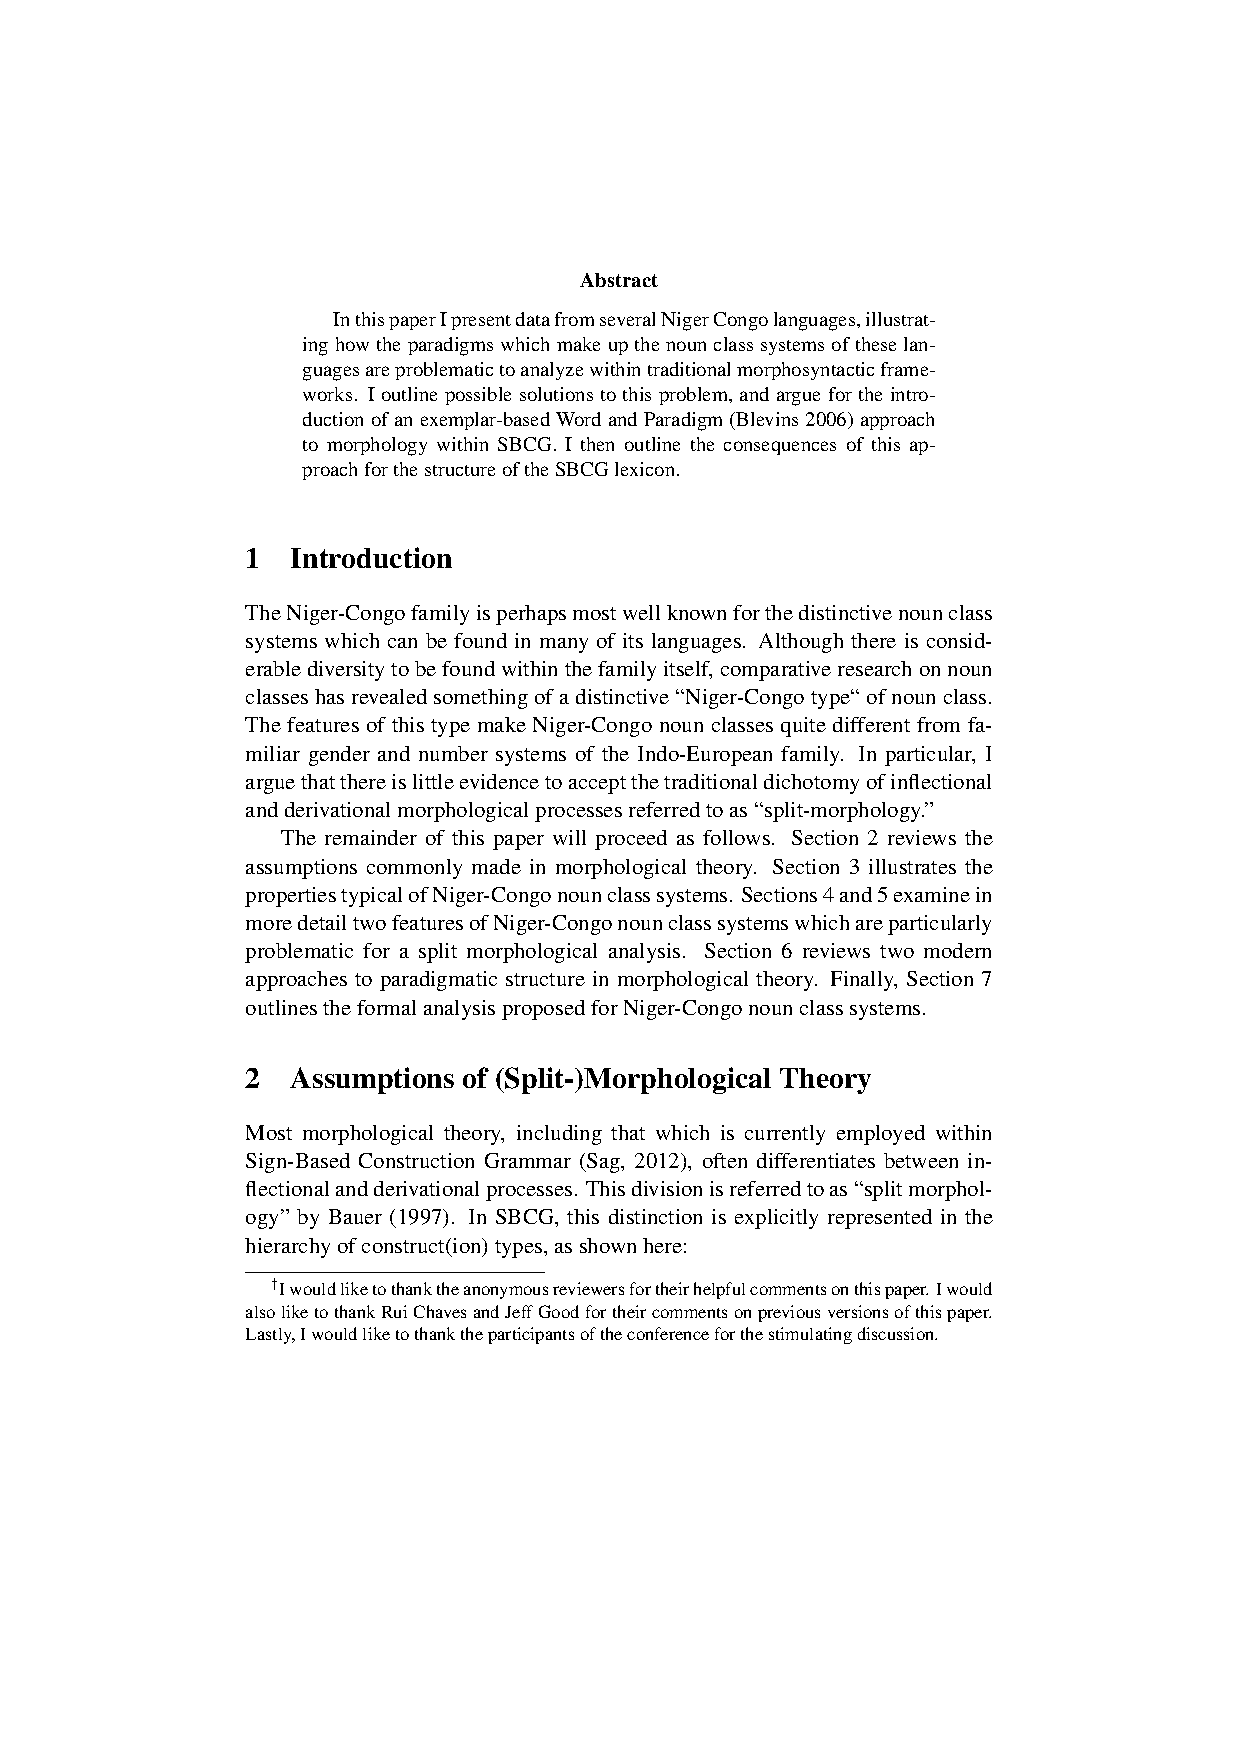
\includepdf[pages=-,pagecommand=\thispagestyle{plain}]{Includes/hepburn-gray.pdf}
        \setcounter{page}{212}
        \phantomsection
        \addcontentsline{toc}{section}{Paul Kay, Laura Michaelis: Partial Inversion in English}
\thispagestyle{empty}

\begin{center}
  {\huge\bfseries Partial Inversion in English\par}

  \bigskip

~\\
\begingroup
\setlength{\leftskip}{0pt plus 1fill}
\setlength{\rightskip}{0pt plus 1fill}
\setlength{\parindent}{0pt}
\setlength{\parfillskip}{0pt}
  \formatauthor{Paul Kay}{\begin{tabular}{@{}c@{}}University of California, Berkeley\end{tabular}}
\formatauthor{Laura Michaelis}{\begin{tabular}{@{}c@{}}University of Colorado Boulder\end{tabular}}

\par\endgroup

  \vspace*{8ex}

  Proceedings of the 24th International Conference on\par Head-Driven Phrase Structure Grammar

  \bigskip

  University of Kentucky, Lexington

  \medskip

  Stefan Müller (Editor)

  \medskip

  2017

  \medskip

  CSLI Publications

  \medskip

  pages 212--216

  \medskip

  \url{http://csli-publications.stanford.edu/HPSG/2017}
\end{center}
\vfill

\noindent
Keywords: Derivation, Locative Inversion, Existential Inversion, Deictic Inversion, SBCG, Focus


\vfill
\noindent
% APA Style
Kay, Paul, \& Michaelis, Laura. 2017. Partial Inversion in English. In Müller, Stefan (Ed.), \emph{{Proceedings of the 24th International Conference on Head-Driven Phrase Structure Grammar, University of Kentucky, Lexington}}, 212--216. Stanford,
CA: CSLI Publications. \hfill\href{http://creativecommons.org/licenses/by/4.0/}{\includegraphics[height=.75em]{Includes/ccby.eps}}

\newpage
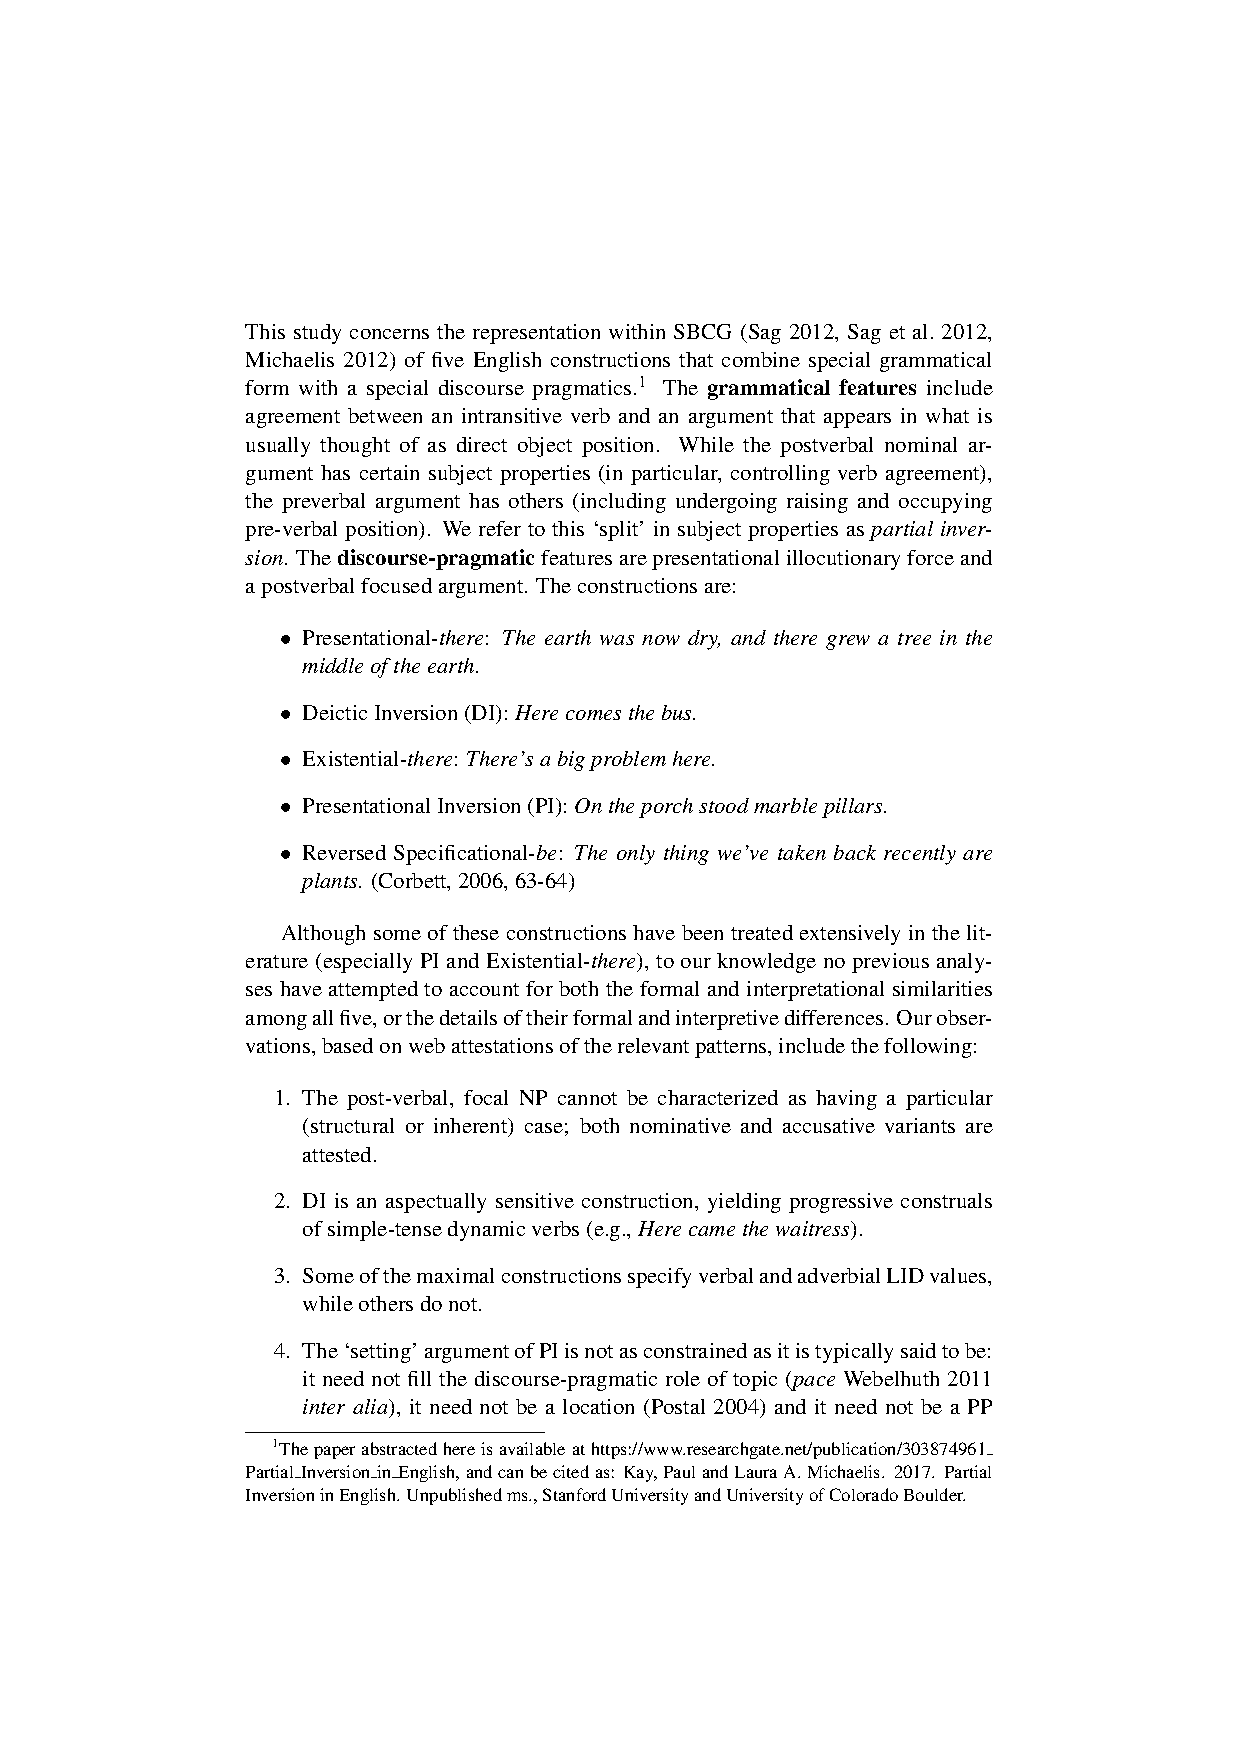
\includepdf[pages=-,pagecommand=\thispagestyle{plain}]{Includes/kay-michaelis.pdf}
        \setcounter{page}{217}
        \phantomsection
        \addcontentsline{toc}{section}{Sarah Hye-yeon Lee: The Syntax of the \emph{not only ... but also ...} Construction}
\thispagestyle{empty}

\begin{center}
  {\huge\bfseries The Syntax of the \emph{not only ... but also ...} Construction\par}

  \bigskip

~\\
\begingroup
\setlength{\leftskip}{0pt plus 1fill}
\setlength{\rightskip}{0pt plus 1fill}
\setlength{\parindent}{0pt}
\setlength{\parfillskip}{0pt}
  \formatauthor{Sarah Hye-yeon Lee}{\begin{tabular}{@{}c@{}}University of Southern California\end{tabular}}

\par\endgroup

  \vspace*{8ex}

  Proceedings of the 24th International Conference on\par Head-Driven Phrase Structure Grammar

  \bigskip

  University of Kentucky, Lexington

  \medskip

  Stefan Müller (Editor)

  \medskip

  2017

  \medskip

  CSLI Publications

  \medskip

  pages 217--232

  \medskip

  \url{http://csli-publications.stanford.edu/HPSG/2017}
\end{center}
\vfill

\noindent
Keywords: HPSG, linearization, not only but also, coordination, correlative coordination, inversion


\vfill
\noindent
% APA Style
Lee, Sarah Hye-yeon. 2017. The Syntax of the \emph{not only ... but also ...} Construction. In Müller, Stefan (Ed.), \emph{{Proceedings of the 24th International Conference on Head-Driven Phrase Structure Grammar, University of Kentucky, Lexington}}, 217--232. Stanford,
CA: CSLI Publications. \hfill\href{http://creativecommons.org/licenses/by/4.0/}{\includegraphics[height=.75em]{Includes/ccby.eps}}

\newpage
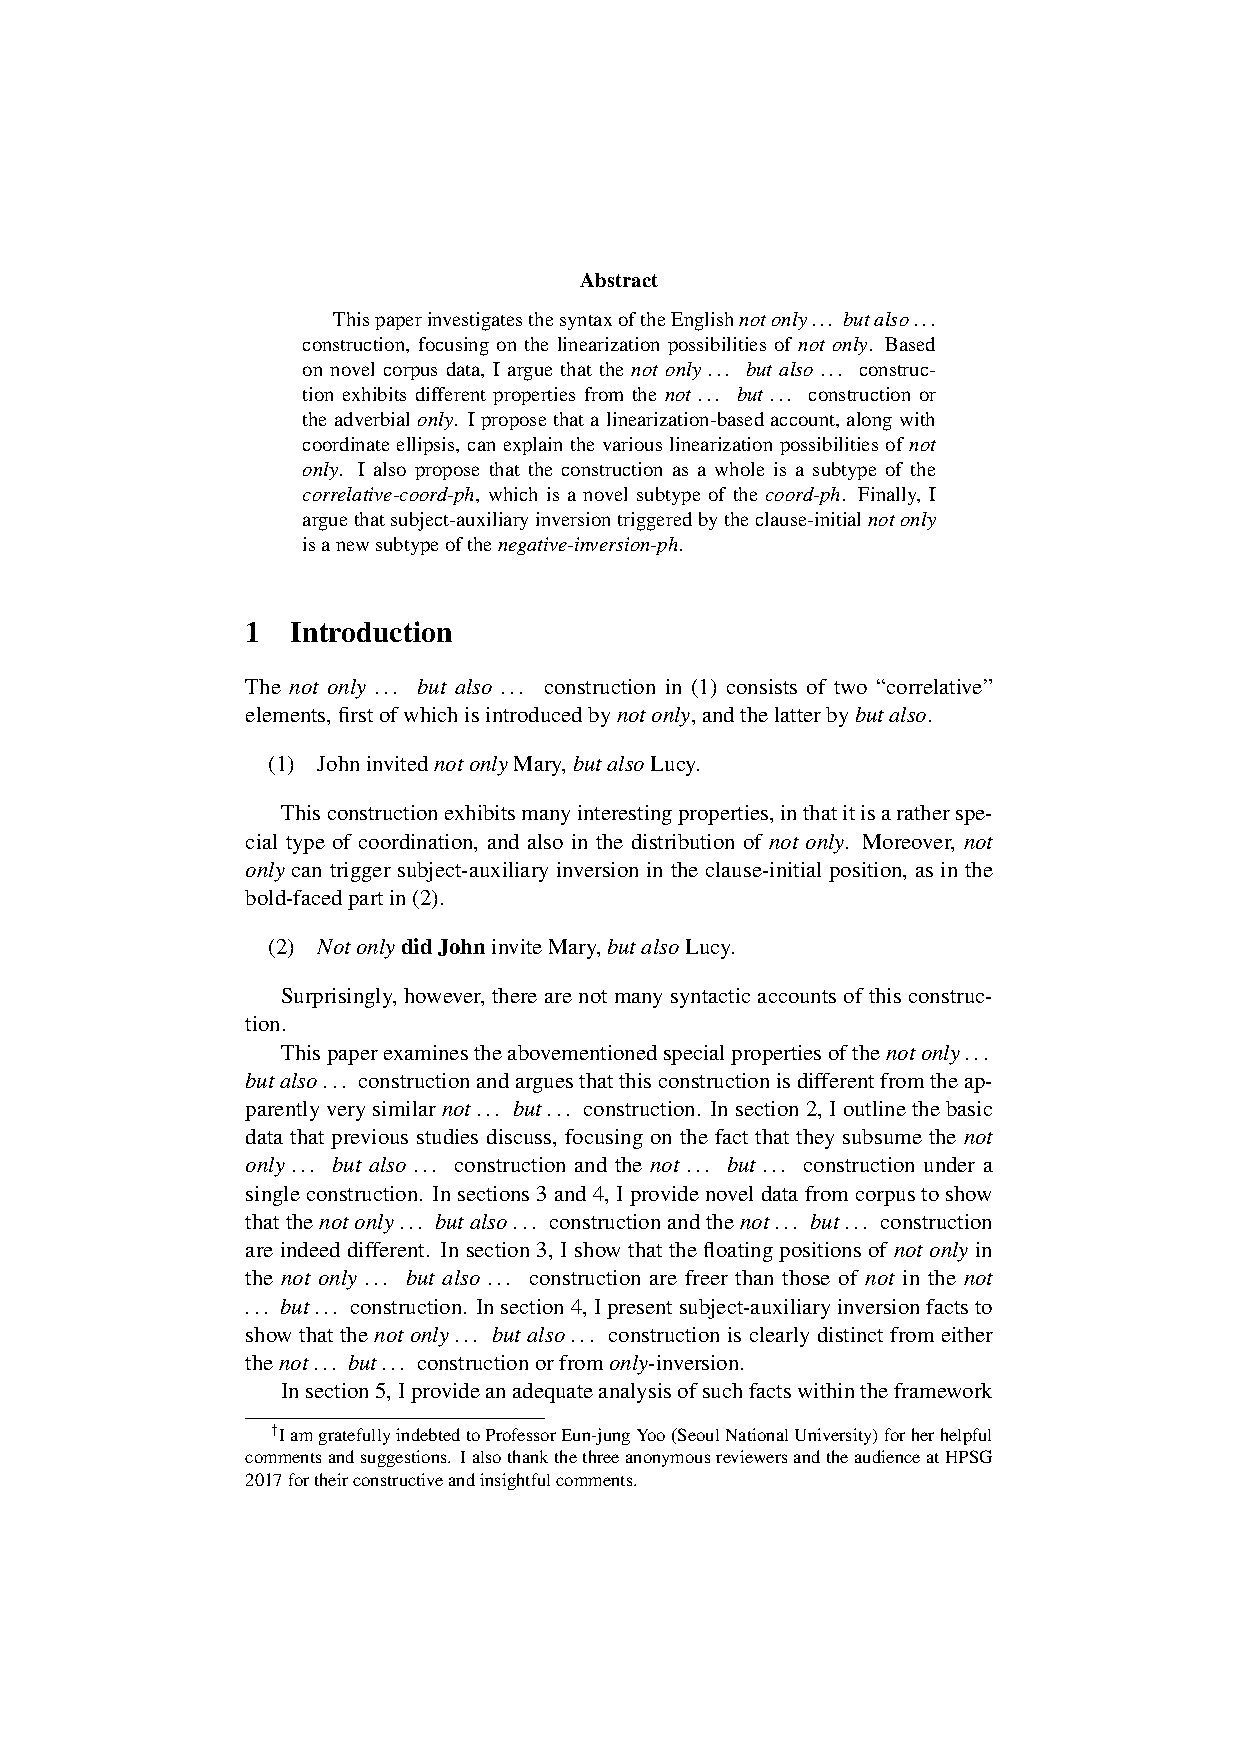
\includepdf[pages=-,pagecommand=\thispagestyle{plain}]{Includes/lee.pdf}
        \setcounter{page}{233}
        \phantomsection
        \addcontentsline{toc}{section}{Takafumi Maekawa: English prepositional numeral 
constructions}
\thispagestyle{empty}

\begin{center}
  {\huge\bfseries English prepositional numeral 
constructions\par}

  \bigskip

~\\
\begingroup
\setlength{\leftskip}{0pt plus 1fill}
\setlength{\rightskip}{0pt plus 1fill}
\setlength{\parindent}{0pt}
\setlength{\parfillskip}{0pt}
  \formatauthor{Takafumi Maekawa}{\begin{tabular}{@{}c@{}}Ryukoku University\end{tabular}}

\par\endgroup

  \vspace*{8ex}

  Proceedings of the 24th International Conference on\par Head-Driven Phrase Structure Grammar

  \bigskip

  University of Kentucky, Lexington

  \medskip

  Stefan Müller (Editor)

  \medskip

  2017

  \medskip

  CSLI Publications

  \medskip

  pages 233--247

  \medskip

  \url{http://csli-publications.stanford.edu/HPSG/2017}
\end{center}
\vfill

\noindent
Keywords: Noun 
phrase syntax, numerals, prepositions


\vfill
\noindent
% APA Style
Maekawa, Takafumi. 2017. English prepositional numeral 
constructions. In Müller, Stefan (Ed.), \emph{{Proceedings of the 24th International Conference on Head-Driven Phrase Structure Grammar, University of Kentucky, Lexington}}, 233--247. Stanford,
CA: CSLI Publications. \hfill\href{http://creativecommons.org/licenses/by/4.0/}{\includegraphics[height=.75em]{Includes/ccby.eps}}

\newpage
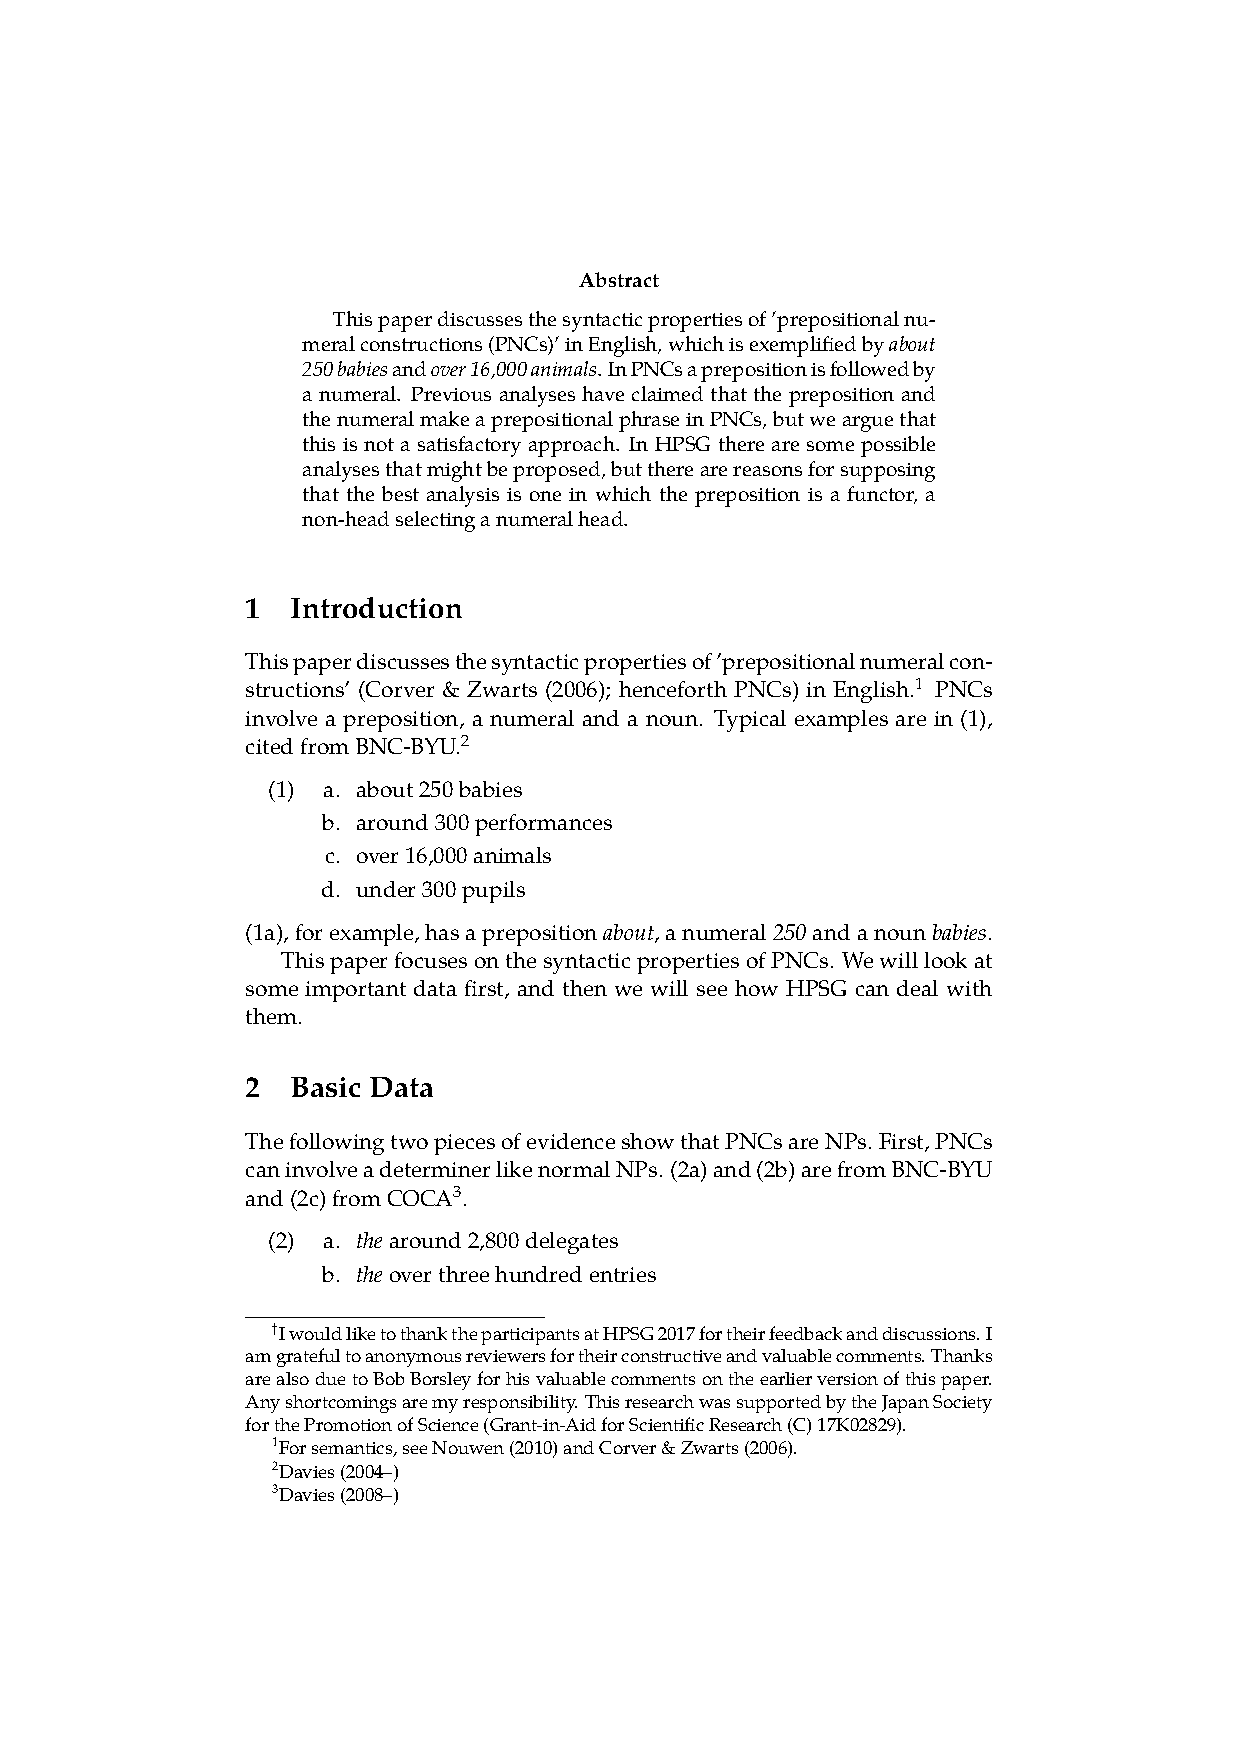
\includepdf[pages=-,pagecommand=\thispagestyle{plain}]{Includes/maekawa.pdf}
\end{document}
